%%% Local Variables: 
%%% mode: latex
%%% TeX-master: "../KanjiHWR"
%%% End: 

\chapter{Handwriting Recognition Engine}
\label{chap:handwritingrecognitionengine}

% %- Why this section? 
% %   The purpose of this section is to describe the software module of the 
% %   HWR engine.
% %   Any important of the software should be described.~This is the core of the
% %   HWR part of the software and therefore needs description.
% %   It would be off purpose, if non-technical aspects of the HWR Engine would be 
% %   described.
% % - What goes into this section?
% %   The main content of this section is the complete functionality of the 
% %   HWR engine.
% %   It should become apparent how the HWR engine works.
% %   * if describing a problem: why is the problem relevant.
% %     The problem of HWR is relevant, because it is the crucial novelty of the
% %     application.~The combination of a Kanji learning tool and a HWR is a new 
% %     thing.~It enables user to practice writing Kanji.~(maybe too high-level for
% %     this section, move to intro / motivation section).
% %   * if describing a solution to a problem: 
% %     what alternatives were there to solve it?    
% %     Instead of a HWR engine, the user could either not have a HWR engine and
% %     write on paper or not practice writing the Kanji.
% %     why was this solution chosen? 
% %     because it creates an additional benefit, that was not available before.
% %     what made it the best choice? 
% %     the fact that it writing on paper is impractical and not practicing does
% %     not lead to the desired result.

% %     was it the optimal solution? given there is only not practicing and
% %     practicing on paper: yes.

% % - How will this section be structured and organised?
% %   The organisational structure of the section is already layed out in the
% %   sections and subsections.
% % - In what style will it be written?
% %   The style of writing will be technical.~A technical description, using
% %   pseudocode.
% % - Next action - what to write first?
% %   The next part to write is the general introduction to this chapter

% %xxx always: what alternatives were there?

% In this chapter the core of the recognition system is going to be presented.
% The other chapters concerning with the system design have a more general focus.
% The present chapter gives an insight into the details of how the handwriting
% recognition is implemented.~The chapter has several sections.~The first section
% briefly presents the data capturing module.~Section~\ref{sec:hwre:dataformat}
% discusses the choice of the data format for both run-time and storage.
% The next section,~\ref{sec:hwre:database} describes the database structure.
% The sections after that are concerned with the actual recognition process.
% The different kinds of stroke matching are discussed in 
% section~\ref{sec:hwre:strokerecognitionprocess}, including dynamic time warping.
% The Radical recognition depends on the stroke matchning and is presented in
% section~\ref{sec:hwre:radicalrecognitionprocess}.
% The character recognition is then a combination of the stroke matching and
% the Radical recognition.~Section~\ref{sec:hwre:characterrecognitionprocess}
% informs about the character recognition.
% The last section~\ref{sec:hwre:errorhandling} of the chapter contains the 
% discussion of the error handling in the system.

% \section{Data Capturing}
% \label{sec:hwre:datacapturing}

% Each handwriting recognition process begins with data capturing.
% The user's handwriting must be captured and fed into the system.~The data 
% capturing is therefore a crucial part of the whole process.~In this system 
% a GUI is used for the capturing of the pen movements on a writing surface.

% %this should deal with how the data are captured during the process
% %mouse coordinates and stuff

% %- Why this section? 
% %  The purpose of this section is to describe the data capturing process.
% %  It would be off purpose, if it describes to much around - the devices, the
% %  transmission.~This should focus on the capturing as such.
% %  It should not go into great deail.
% %  
% %- What goes into this section?
% %  The main content of this section is the technical data capturing.
% %  A description of how to
% %  programmatically generate a pen trajectory from reading mouse coordinates.
% %  
% %  * if describing a problem: why is the problem relevant.
% %    The relevance of the problem is evident: Without the user's writing,
% %    there would not be any handwriting recognition.
% %
% %  * if describing a solution to a problem: what alternatives were
% %    there to solve it, why was this solution chosen? 
% %    The alternatives are not massively relevant here, since they come down
% %    to using different input devices, which is discussed elsewhere.
% %
% %    what made it the best choice? 
% %    the fact that this is just how it is done.
% %    was it the optimal solution?
% %    yes.
% %
% %- How will this section be structured and organised?
% %  The organisational structure of the section begins with describing the mobile 
% %  input GUI from a technical level.
% %  Then the class in the background that actually captures the mouse events.
% %  the capturing of the mouse events.
% %  the storing of the data points in lists.
% % 
% %- In what style will it be written?
% %  The style of writing will be technical.~using pseudocode if required.
% %  however the algorithm is not relevant here.
% %
% %- Next action - what to write first?
% %  The next part to write is the one about the GUI
% %  also the substructuring needs to be done as required.~DONE

% \subsection{Writing Surface} %the mobile GUI
% \label{sec:hwre:writingsurface}
% %NEXT ACTION - describe writing surface and it's GUI

% The writing surface module, the view is split into two parts: The writing 
% surface GUI and the writing surface background module. The technical design of 
% the data input GUI is described in 
% section~\ref{sec:arch:handwritingdatainputview}.

% \subsubsection{Writing Surface GUI}
% \label{sec:hwre:writingsurfacegui}
% The GUI works with pen-down and pen-up events. It has a cross in the middle in 
% order to partition the writing surface the same way that character practising 
% paper sheets are usually partitioned.~The GUI class is listening to 
% \emph{pen-down}, \emph{pen-up} and \emph{pen-move} events.
% These are the equivalent events on 
% mobile devices for regular mouse-down, mouse-up and mouse-move events.~
% However, there is one difference - the pen-move event can only be captured 
% between a pen-down and a pen-up event.~
% An earlier conceptual idea for the HWR engine included using the
% mouse-move events during the input of a character between the strokes.~This 
% could not be realised, however, because the series of pen-move events can only 
% be captured when there has been a previous pen-down event before a pen-up event.~

% xxx
% why could it not be realised?
% physical contact of pen to writign surface.

% The GUI captures the events and passes the point coordinates on to 
% the background class.

% \subsubsection{Writing Surfaces Background Module}
% \label{sec:hwre:writingsurfacebackground}

% When a pen-down event is detected, the background class of the GUI starts 
% listening for the pen movement.~All point coordinates and the time of their 
% capturing are stored in two separate lists with the same indices.
% An alternative solution would have been to store a number of instances of a 
% custom-made encapsulated \emph{Point} 

% xxx look for class names in whole chapter and make them cursive.


% class including the time stamp in one 
% list only, however, using two separate lists resulted in increased speed.
% Therefore, the point coordinates are stored in the frameworks Point class that 
% does not account for time stamps.~Therefore a separate list is used for the 
% timestamps only.

% The background module of the writing surface mainly administrates the capturing 
% of the pen trajectory and sends it to the recognition module as soon as a 
% stroke is finished.~Therefore the system does not receive a separate signal 
% indicating that the drawing of the character is finished.~That design creates 
% segmentation problem that is solved with the \emph{clear} button and the 
% \emph{clear} message.~The segmentation of characters is left undetermined - only 
% the beginning of it is determined through the \emph{clear} message that is sent 
% to the mobile view from the controller - or the clear message that is sent to 
% the controller because the user clicked the \emph{reset} button.
% After a stroke is finished the corresponding point and timestamp sequences are 
% passed to the main part of the HWR engine.~

% \section{Data Format}
% \label{sec:hwre:dataformat}

% % - Why this section? 
% %   The purpose of this section is to give the reader an idea of how the captured
% %   data is structured.~That means concretely the character format, describing
% %   the HW trajectories.~This is necessary in order to be able to explain the
% %   mode of operation of the HWR engine in detail.

% %   It would be off purpose, if the section contained a description of the 
% %   lexical data, which is described in a different section.

% % - What goes into this section?
% %   The main content of this section is what is stated under purpose:
% %   A description of how the captured data is structured.

% %   * if describing a problem: why is the problem relevant.
% %     The task of handwriting recognition is essentially a task 
% %     working with data.
% %     Therefore the structure of the data is one of the crucial points.
    
% %   * if describing a solution to a problem: what alternatives were
% %     there to solve it, why was this solution chosen? 

% %     The solution was chosen because of its clarity, simplicity and 
% %     accessibility, also because of its interoperability with potential 
% %     other systems.
% %     what made it the best choice? was it the optimal solution?
% %     For the purpose followed with the system - yes, it was the optimal solution,
% %     because it does not require much effort to parse the stored data
% %     and it contains all necessary information in a structured manner.
    
% % - How will this section be structured and organised?
% %   The organisational structure of the section contains:

% %   A general description of the XML format - why it was used as opposed to
% %   other possible formats like unipen and inkml.
% %   show requirements!
% %   show process of how I came to current data formats.
% %   include character models 1-4 on pages.~- however, not everything in one go,
% %   but rather in the individual sections if possible.
% %   in the end, a radical has its own format that is unchanged, even
% %   if internal structure of a stroke is changed.
% %   (unipen is only text based, inkml does not help here, but the system allows
% %   for exchange of the custom format with those)

% %   data format of and representation of 
% %   point, stroke, box, radical, character s.~20-23, 25f

% % - In what style will it be written?
% %   The style of writing will be technical - a description of the XML format.
% %   Pointer to code sample in Appendix.

% % - Next action - what to write first?
% %   The next part to write is the actual subsection 
% %   structure of this section.~DONE
% %   Think about requirements and write them down.


% \subsection{Requirements of the Data Format}
% \label{sec:hwre:requirementsofdataformat}

% %show requirements!
% %think about differences between static data format and runtime data format.

% The data format for the recognition process underlies a number of requirements.
% Firstly, it has to be stated that two main data formats are necessary.~
% One for the actual recognition process as a data structure in RAM.
% Secondly, there needs to be a storage format for the data base that represents
% the handwriting of a character, radical, stroke, point list or simple point.
% The requirements for both data structures are:
% \begin{itemize}
%   \item \textbf{Expressiveness}: The data structure should be able to 
%         fully represent a complete character and all sub-elements that belong 
%         to it.~That requirement is due to the structural approach to handwriting
%         recognition that is the basis for the error handling.

%   \item \textbf{Well-definedness}: The information structure should be 
%         unambiguous, two different characters must have a different structure.
% \end{itemize}
% The storage structure has some additional requirements:
% \begin{itemize}
%   \item \textbf{Accessibility}: The data should be formatted in a way that a 
%         human editor can access the data, but it should also be prepared for 
%         programmatic access.
%   \item \textbf{Well-formedness}: There should be a way to check if the data is 
%         well-formed
%   \item \textbf{Parsabilty}: It should be possible to create the run-time data 
%         structure from the storage data structure.
% \end{itemize}
% The run-time data structure should in addition provide
% \begin{itemize}
%   \item \textbf{Serialisability}: It must be possible to create the storage 
%         data structure from the run-time data structure.
% \end{itemize}
% Any combination of two formats used should meet the above requirements, 
% at best in a uniform way.~That is, any combination of storage format and 
% run-time format should ideally be compatible without the need of a complex
% data format converter.

% %xxx how much do I really have to say about the unipen format?
% %xxx does it really not meet the requirements?

% % Both:
% % \emph{expressiveness}
% % \emph{well-definedness}

% % Storage:
% % \emph{accessibility}
% % \emph{well-formedness}
% % \emph{parsabilty}

% % Run-time:
% % \emph{serialisability}

% \subsection{Existing Handwriting Formats}
% \label{sec:hwre:existingformats}

% There are some existing formats for the description of handwriting.~Their 
% intended use is for handwriting recognition systems.~The formats that will be
% reviewed in this section are the \emph{Microsoft ISF} format in 
% section~\ref{sec:hwre:msisfformat}, which is a binary format.
% The other formats are text based and human-readable.~In this short review,
% the formats will be checked against the requirements defined in 
% section~\ref{sec:hwre:requirementsofdataformat}. We will consider 
% \emph{InkML} in section~\ref{sec:hwre:inkml}, 
% \emph{UNIPEN} in section~\ref{sec:hwre:standardunipenformat}, 
% \emph{hwDataset} in section~\ref{sec:hwre:hwdataset} and 
% \emph{UPX} in section~\ref{sec:hwre:unipenformatupx}.
% The central question is, if one of these formats meets the above requirements in 
% a sufficient way.~This is unclear, because the most of the formats have been 
% originally developed mainly for alphabetic scripts or for usage scenarios 
% different from the one proposed in this chapter.

% \subsubsection{The Microsoft Ink Serialized Format (\emph{ISF})}
% \label{sec:hwre:msisfformat}

% The \emph{Ink Serialized Format} (ISF) format is owned by the 
% Microsoft Corporation.~However, it is not a proprietary format, the 
% specification is freely available.~Since the format is purely binary, 
% it can not meet one of the requirements for the storage data structure:
% It is not feasible for a human to read and write files in that format,
% therefore ISF does not provide the necessary 
% \emph{accessibility}~\shortcite{Microsoft2007}.~The format could still be used 
% as a run-time data structure, if it meets the requested criteria.
% The requirement of \emph{serialisability} is generally met.~A binary format 
% allows for fast and reliable programmatic access to the data, it can be stored
% in binary files on a data storage medium.~The problem that accrues from this 
% type of serialisation is that the storage format, the format used in a file or 
% database, would again not be human-editable and therefore fail to meet the 
% \emph{accessibility} requirement.~
% In order to provide a serialisation that results in a human-readable format, 
% a format converter would be needed.~Another problem originates from the 
% ISF format specification: \\
% It accounts only for the description of mouse coordinates or pen trajectories, 
% but does not offer any structures for linguistic information.~
% It fails to meet the ideal, a unified format for linguistic and graphic 
% information, as it is lacking some degree of \emph{expressiveness}.

% \subsubsection{InkML}
% \label{sec:hwre:inkml}

% InkML is a markup language for describing electronic pen trajectories.~
% Hence the name \emph{Ink}. The letter combination \emph{ML} stands for markup 
% language, as is customary 
% for XML-based and SGML-based languages.~The specification is currently in a 
% draft status, maintained by the World Wide Web Consortium 
% (W3C)~\shortcite{W3C2006}.
% Judged from the viewpoint of the defined requirements, InkML is a candidate
% for the storage format. As an XML format with an XML schema it fulfils the 
% criterion of \emph{well-formedness} by design: 
% Any piece of InkML code can be evaluated automatically with common techniques, 
% since InkML has a well-defined scheme description.

% The main XML elements in the simplest form of InkML are 
% the \textbf{<ink>}- and the \textbf{<trace>}-element.
% These elements allow for a very simple form of a pen trajectory, 
% basically a flat list of point coordinates.
% The <ink>-element is the root element of any InkML code. 
% The <trace>-element holds point coordinates.
% \begin{xmlcode}
%   \begin{lstlisting}[emph={trace,timestamp,channel},
%                      emphstyle=\color{blue}\textbf,
%                      emph={[2]name,type,units,respectTo,time,
%                               timeOffset,timestampRef},
%                      caption={Demonstration of the \emph{time channel} and the \emph{trace} tag},
%                      label=lst:TraceTag]
%     <ink>
%       <timestamp xml:id="ts001" 
%                  time="1265122414000"/>

%       <timestamp xml:id="ts002" 
%                  timeOffset="600000" 
%                  timestampRef="#ts001"/>

%       <traceFormat xml:id="0001_tf">
%         <channel name="X" type="decimal" />
%         <channel name="Y" type="decimal" />
%         <channel name="T" 
%                  type="integer" 
%                  units="ms" 
%                  respectTo="#ts001" />
%       </traceFormat>

%       <trace>
%         282  45 100, 281  59 100, 284  73 200, 285  87 200, 287 101 300, 
%         288 115 300, 290 129 400, 291 143 500, 294 157 500, 294 171 600
%       </trace>
%     </ink>
%   \end{lstlisting}
% \end{xmlcode}
% Listing~\ref{lst:TraceTag} covers the general gist of the InkML format.
% Despite being an XML format, it is a flat format, each value triple, 
% separated by commas, represents one point in a coordinate notation and
% an offset to a time stamp.

% In order to add \emph{time} information to the trace,
% a time channel needs to be defined. Listing \ref{lst:TraceTag} shows the 
% definition and use of a time channel in the beginning. 
% The example shows a time channel whose values for a given point are the 
% relative to the timestamp referred to by 
% \emph{\#ts001}~\shortcite{W3C2006}. There are two \emph{timestamp} tags.
% The first one has the ID \emph{ts001} and is referred to by both the
% time channel and the second time stamp that defines a time offset to time stamp
% \emph{ts001} with the \emph{timeOffset} attribute.
% The possibility to define time channels enables the InkML format to hold 
% information about the time at which a sample point has been taken.
% This is useful for the recognition mechanism used in this application,
% because it compares point coordinates as well as time stamps.
% The InkML data structure fulfils several of the requirements necessary for a 
% storage data structure.~InkML is 
% \begin{itemize}
%   \item \textbf{well-defined}: Any point sequence that has different coordinate
%         values than another point sequence can be distinguished from the other.
        
%   \item \textbf{accessible}: As an XML format it can be handled programmatically,
%         but is also human-readable and can be edited by a human with a simple
%         interface like a text editor.

%   \item \textbf{well-formed}: As an XML format it can be validated according to 
%         it's specification.

%   \item \textbf{parsabale}: As an XML format, InkML does not need to be parsed 
%         with custom-made methods, since most modern high-level languages offer
%         an access method to XML tree structures.
% \end{itemize}
% However, InkML is lacking some \emph{expressiveness}. Only pen trajectories and
% their time stamps can be expressed in the InkML format. InkML is not designed 
% to hold any of the other information compulsory for the structural handwriting
% recognition.~In the case of character recognition, it needs to be able to 
% account for more than coordinate points and time stamps.~There needs to be a 
% way to encode structural information about the characters and sub-elements of 
% the characters. InkML does not seem to be a sufficient format for the given task.

% \subsubsection{The Standard UNIPEN Format}
% \label{sec:hwre:standardunipenformat}

% The standard UNIPEN format specification is a file format definition for a flat
% text file.~It contains tags in dot-notation. For example the tag \emph{.COMMENT}
% means that the following free text should be ignored, the tag \emph{.KEYWORD} 
% is used to define a new keyword, while the tag \emph{RESERVED} states that
% the text that comes after that tag is a reserved word within the UNIPEN format.
% The format is self-defined with the three keywords above. Any new keyword is
% defined with \emph{.KEYWORD}~\shortcite{Guyon1994,Unipen}.

% As a data structure for the purpose of a handwriting recognition, UNIPEN can 
% serve as a storage format, which is the primary purpose for the existence of the
% format. The UNIPEN format accounts for both pen trajectories as well as 
% information about the characters that have been written.
% \begin{xmlcode}
%   \begin{lstlisting}[emph={COMMENT,COORD,SEGMENT},emphstyle=\textbf,caption={Demonstration of the \emph{UNIPEN} format},label=lst:unipen]
% .COMMENT #################################################################### 
% .COORD   X Y

% .SEGMENT TEXT 235:0-297:9 OK "Kurosu Masaaki"
% .SEGMENT CHARACTER 235:0-255:9 OK  "JISx3975_'Kuro'"

% .PEN_DOWN 
%   486 -1456 
%   488 -1454 
%   490 -1452 
%   488 -1450 
%   488 -1450 
%   486 -1452 
%   480 -1456 
%   474 -1466 
%   464 -1480 
%   452 -1492 
%   440 -1506 
%   428 -1524
% .PEN_UP 
%   406 -1556 
%   394 -1574 
%   384 -1590 
%   374 -1602
% .PEN_DOWN 
%   \end{lstlisting}
% \end{xmlcode}
% Listing~\ref{lst:unipen} is an excerpt from a data file created 
% by~\shortciteANP{Unipen}~\citeyear{Unipen}. It shows an example of a UNIPEN data structure.
% The \emph{.COORD} tag defines the structure of the pen coordinates. 
% The \emph{.SEGMENT} tag with the \emph{TEXT} modifier informs about the
% full text of the next number of segments. The \emph{.SEGMENT} tag with the
% \emph{CHARACTER} modifier informs about the character that is represented
% with the sequence of pen coordinates. The other information given is the
% start and end position within the file and the character code in JIS encoding.
% The \emph{.PEN\_DOWN} tag can be understood as a flag. All pen coordinates 
% following this tag have been captured as \emph{pen down} coordinates.
% The tag \emph{.PEN\_UP} sets the opposite flag: The coordinates stated after 
% this tag were captured while the pen was not touching the writing surface.
% The last \emph{.PEN\_DOWN} tag is the beginning of a new coordinate sequence
% for the next stroke. From a requirements point of view the UNIPEN provides a
% high standard, as it meets a great number of requirements for the storage 
% structure. \\
% The UNIPEN format is:
% \begin{itemize}
%   \item partially \textbf{expressive}: UNIPEN can represent a complete character
%         and the pen trajectory along with it. It does however, not account for
%         capturing the time information. At a constant sample rate the time stamps
%         of the individual points could theoretically be calculated, 
%         if time stamp of the first point is encoded in the meta information. 
%         However, that solution is not optimal, because it needs constant
%         sampling, even between a \emph{pen-up} and a \emph{pen-down} event.
%         There are input devices that do not offer those coordinates and the 
%         recognition system presented here does not rely on them for that reason.
%         The examples given are encoded in JIS, but it seems possible and feasible
%         to use the format with Unicode encoding.

%   \item \textbf{well-defined}: The UNIPEN is unambiguous, two different 
%         characters do have a different data structure, because the JIS code 
%         can serve as an ID.

%   \item \textbf{accessible}: The data resides in flat text files, designed for 
%         human editing. It is accessible programmatically, too, but has a weakness
%         on that requirement compared to an XML-based format.

%   \item \textbf{parsable}: The flat file format can be parsed easily. Due to its
%         procedural nature it is also possible to create a run-time data structure
%         that is conceptually based on the storage structure and therefore
%         serialisable.
% \end{itemize}
% The main weakness of the flat format file is the lack of \emph{well-formedness}.
% There is no automatic way to check a document against a predefined format 
% specification. It can not be assessed if a file is well-formed.
% Additionally, the expressive power of the UNIPEN format would be seriously 
% challenged if it should provide for sub-structures of characters.
% In order to do so, it would be necessary to create new tag definitions for the 
% Radicals of the Kanji.~\shortciteANP{Agrawal2005}~\citeyear{Agrawal2005} 
% describe some more shortcomings of the UNIPEN format. It can be concluded that 
% the standard UNIPEN format is not suitable for the task given. 

% \subsubsection{Handwriting Dataset (\emph{hwDataset})}
% \label{sec:hwre:hwdataset}

% The \emph{Handwriting Dataset} (hwDataset) is an XML format that is a complement
% to InkML. It is inspired by the UNIPEN format. The \emph{hwDataset} format 
% attempts to close the gap between pure ink data and the annotations that are 
% needed for handwriting recognition~\shortcite{Bhaskarabhatla2004}. 
% The format contains three main parts. The \emph{datasetInfo}, 
% the \emph{datasetDefs} and the \emph{hwData}. The datasetInfo element holds
% any metadata, like \emph{name}, \emph{category} and the like.
% The dataSetDefs encompasses information about \emph{data sources}, different
% \emph{writers} and their features like \emph{handedness}, \emph{gender}, 
% \emph{age}. The \emph{hwData} element in the XML code organises the 
% handwriting data hierarchically. Each hierarchy level contains one or 
% more \emph{hwTrace} elements. The hwTrace element refers to an InkML file, 
% containing the actual handwriting data. A detailed description of the hwDataset 
% format can be found in~\shortciteANP{Bhaskarabhatla2004}~\citeyear{Bhaskarabhatla2004}. 

% The format provides an XML scheme description and thus meets the 
% \emph{well-formedness} requirement. It is \emph{well-defined}, 
% because it accounts for unique structures. The \emph{parsabilty} is not an 
% issue for any XML format, since methods for accessing XML trees are provided 
% by modern programming libraries.
% The \emph{accessibility} is provided, the format has a clearly defined structure
% that can easily be understood by humans.
% The hwDataset format can structure many desirable information for the handwriting
% learning system proposed in this chapter. 
% From an \emph{expressiveness} viewpoint it can create substructures for 
% different parts of a sequence of pen trajectories. The \emph{hierarchy level} (H)
% of a trace accounts for the expressive power necessary. The H(n) elements 
% of the hwData elements are designed to hold meaningful names like 
% \emph{PARAGRAPH} or \emph{WORD}. It may be possible to use the format even to 
% denote different parts of the same character. There is no reason why one should
% not introduce an H(n) definition for \emph{RADICAL} or \emph{GRAPHEME}.

% \subsubsection{The UNIPEN XML Format (\emph{UPX})}
% \label{sec:hwre:unipenformatupx}

% The format \emph{Unipen for XML} (UPX) can be seen as an XML version of the
% UNIPEN format. The UNIPEN standard described in 
% section~\ref{sec:hwre:standardunipenformat} does not bear any resemblance
% with the InkML format shown in section~\ref{sec:hwre:inkml}.
% Both formats fulfil a number of the requirements presented in 
% section~\ref{sec:hwre:requirementsofdataformat}, but both formats fail to 
% fulfil them all. The hwDataset format described in 
% section~\ref{sec:hwre:hwdataset} solves many of the problems UNIPEN faces,
% as it brings together a superset of the expressiveness of UNIPEN with
% the well-defined InkML format in a uniform way.
% According to~\shortciteANP{Agrawal2005}~\citeyear{Agrawal2005} hwDataset
% was designed to support new data collection. The motivation to create another
% format came about from the fact that existing UNIPEN resources should be made
% available in a modern XML-based format that unifies InkML and UNIPEN.
% hwDataset comes very close to this aim, but does not necessarily account for a 
% conversion of UNIPEN resources. 
% \shortciteANP{Agrawal2005}~\citeyear{Agrawal2005} attempt to create a format 
% that allows for a well-defined conversion from UNIPEN.
% The UNIPEN foundation considers UPX as the new de facto standard format for 
% storing annotated databases of on-line pen input~\shortcite{UnipenConsortium2006}.

% UPX is a multi file format. It resembles hwDataset in the way that it comprises 
% both meta information and data annotations as well as pure InkML data in 
% separate files. Within the UPX \emph{hwData} element there can be any number
% of \emph{hLevel} elements in order to define the hierarchy of the trajectory.
% Listing~\ref{lst:hLevelinupx} shows an example 
% after~\shortciteANP{UnipenConsortium2006}~\citeyear{UnipenConsortium2006}. In the listing, the \emph{hLevel} tag
% is demonstrated. The word \emph{sexy} is described hierarchically.
% Firstly, in the outermost \emph{hLevel} tag, the \emph{level} attribute specifies
% a \emph{WORD}. Then the inner \emph{hLevel} elements specify a lower level
% of hierarchy, the characters. Note that not all characters are defined
% individually in this example.
% The \emph{hwTraces} elements surround a number of \emph{traceView} elements that
% in turn point to the corresponding positions in an InkML file that holds the 
% pen trajectory. The meta data information that can be stored in UPX has a 
% similar expressive power as the hwDataset format.
% \shortciteANP{Madhvanath2006}~\citeyear{Madhvanath2006} give a full format 
% description of the UPX format in their technical report.

% \begin{xmlcode}
%   \begin{lstlisting}[emph={hLevel,hwTraces},
%                      emphstyle={\color{blue}\textbf},
%                      emph={[2]id,level},
%                      emphstyle={[2]\color{red}},
%                      caption={Demonstration of the \emph{hLevel} tag in UPX},
%                      label=lst:hLevelinupx]
%     <hLevel id="WORD_0" level="WORD">
%       <label id="WORD_0">
%         <alternate rank="1" score="1"/>sexy</alternate>
%       </label>
%       <hwTraces> 
%         <inkml:traceView traceRef="w0629.inkml#dataSet_0_traces" 
%                          from="22" 
%                          to="24"/>
%       </hwTraces>

%       <hLevel id="CHAR_0" level="CHAR">
%         <label id="CHAR_0">
%           <alternate rank="1" score="1"/>e</alternate>
%         </label>
%         <hwTraces> 
%           <inkml:traceView traceRef="w0629.inkml#dataSet_0_traces" 
%                            from="22:91" 
%                            to="22:161"/>
%         </hwTraces>
%       </hLevel>

%       <hLevel id="CHAR_1" level="CHAR">
%         <label id="CHAR_1">
%           <alternate rank="1" score="1"/>y</alternate>
%         </label>
%         <hwTraces> 
%           <inkml:traceView traceRef="w0629.inkml#dataSet_0_traces" 
%                            from="24:61" 
%                            to="24:162"/>
%         </hwTraces>
%       </hLevel>
%     </hLevel>
%   \end{lstlisting}
% \end{xmlcode}

% It seems as if the UPX format was able to fulfil all requirements.
% The UPX format fulfils the requirements of
% \begin{itemize}
%   \item \textbf{Well-definedness}: As an XML structure providing IDs and names 
%         for each element and substructure, the format is well-defined.

%   \item \textbf{Accessibility}: As an XML format it is both human and machine
%         readable and editable.

%   \item \textbf{Well-formedness}: As an XML format with a defined scheme it can
%         be validated for its syntactic features.

%   \item \textbf{Parsabilty}: As an XML format it can be easily parsed into a
%         tree structure.

%   \item \textbf{Expressiveness}: The format provides the missing link between the
%         standard UNIPEN format and the InkML format. Additionally, it can 
%         describe hierarchical structures.
% \end{itemize}
% Since any XML format translates directly into a tree structure, the data 
% structure for the run-time does not need to be defined separately.
% Converting pen trajectories in InkML format into a data stream has been 
% studied~\shortcite{Keshari2008}. These techniques however, are not necessary 
% for the proposed system. The data exchange is provided as technique available
% within the framework without any conversion (see 
% section~\ref{sec:arch:webservice}).

% \subsection{Data Format Description}
% \label{sec:hwre:dataformatdescription}

%   % A general description of the XML format - why it was used that way,
%   % given the requirements

%   % data format of and representation of 
%   % point, stroke, box, radical, character s. 20-23, 25f

%   % show process of how I came to current data formats.
%   % include character models 1-4 on pages. - however, not everything in one go,
%   % but rather in the individual sections if possible.
%   % in the end, a radical has its own format that is unchanged, even
%   % if internal structure of a stroke is changed.
%   % (unipen is only text based, inkml does not help here, but the system allows
%   % for exchange of the custom format with those)

% The data format description could trivially be described with the UPX 
% description. In this case however, UPX needs to be adapted to the special needs.
% This section describes the adaption of UPX to the requirements of an on-line
% handwriting recognition for Kanji characters in a learning environment.
% The section describes both the file format and the run-time data structure.
% xxx further corrections from here downwards xxx

\subsubsection{Point Data Format}
\label{sec:hwre:pointdataformat}

In UPX, points are not represented directly, but in an outsourced InkML file,
where they are part of the InkML standard pen trajectory definition. In InkML
files, points are stored in traces as specified in the InkML format description.
\begin{xmlcode}
  \begin{lstlisting}[emph={traceFormat,channel,timestamp},
                     emphstyle=\color{blue}\textbf,
                     emph={[2]name,type,units,respectTo,id,time},
                     emphstyle={[2]\color{red}},
                     caption={Definition of the trace format},
                     label=lst:traceformat]
    <timestamp xml:id="ts001" 
               time="1265122414000"/>
    <traceFormat xml:id="KanjiStrokeTrace">
      <channel name="X" type="decimal" />
      <channel name="Y" type="decimal" />
      <channel name="T" type="integer"
                        units="ms"
                        respectTo="#ts001" />
    </traceFormat>
  \end{lstlisting}
\end{xmlcode}
Listing~\ref{lst:traceformat} shows the trace format description as used in
the system. The format consists of three channels that are given in ordered 
sequence. There are no intermittent channels. The first two channels are \emph{X}
and \emph{Y} for the pen coordinates. The third channel is \emph{T} for a time 
stamp. The pen coordinates can be given as \emph{decimal} numbers, while the
time stamp (in milliseconds) must be an \emph{integer}.
The \emph{respectTo} attribute in the time channel indicates that all values
must be interpreted as offsets to the time stamp with the id \emph{ts001}.

An actual trace would then contain three values, each value triple separated by
a comma. The trace format definition ensures the correct interpretation of the 
values.
\begin{xmlcode}
  \begin{lstlisting}[emph={trace,channel},
                     emphstyle=\color{blue}\textbf,
                     emph={[2]name,type,units,respectTo,id},
                     emphstyle={[2]\color{red}},
                     caption={A sample trace},
                     label=lst:traceinterpreation]
    <trace id="id123abc">
      45 76 0, 3 5 100, 4 -8 200, 4 -5 300,
      9 -2 400, ...
    </trace>
  \end{lstlisting}
\end{xmlcode}
Listing~\ref{lst:traceinterpreation} shows a trace. Given the file contains
the trace format definition shown in listing~\ref{lst:traceformat}, the trace 
in listing~\ref{lst:traceinterpreation} is interpreted in 
table~\ref{table:sampletraceinterpretation}. 

\begin{table}[htbp]
\begin{center}
  \begin{tabular}{|l||l|l|l|p{200pt}|}
    \hline
    Trace & Channel X & Channel Y & Channel T & Comment \\
    \hline
    45 76 0 & 45 & 76  & 1265122414000 & The first trace initialises 
                                         the values. The time stamp value is
                                         read from timestamp \emph{ts001}. \\
    \hline
    3 5 100 & 48 & 81 &  1265122414100 & The delta values are added to the
                                         existing data. \\
    \hline
    4 -8 200 & 52 & 73 &  1265122414200 & The time stamp values are relative to
                                          \emph{ts001}, not to the last time 
                                          stamp, unlike the pen coordinate 
                                          deltas that are added to the current 
                                          value trace by trace. \\
    \hline
    4 -5 300 & 56 & 68 &  1265122414300 & Negative values are treated as regular
                                          delta values. \\
    \hline
    9 -2 400 & 65 & 66 &  1265122414400 & The values change as expected. \\
    \hline
  \end{tabular}
\end{center}
\caption{Sample trace interpretation}
\label{table:sampletraceinterpretation}
\end{table}

% \paragraph{The run-time data structure} for a point holds the coordinate values 
% and an integer value for the time stamp. The conversion between the run-time 
% instance and the trace format is trivial and needs no description.

% \subsubsection{Stroke Data Format}
% \label{sec:hwre:strokedataformat}

% There is no explicit format for a stroke in the storage structure.
% A stroke is simply the trace between a pen-down event and the following pen-up
% event. All the points captured between form one stroke.

% xxx was bedeutet das im zusammenhang mit der struktur im RAM?
% warum jetzt simply a trace? das steht vorher schon da:
% Thus, in the InkML file format a stroke is simply a trace.


% If a greater number of strokes comes together, each one of them will be a trace
% and they can be grouped together as a \emph{tracegroup} element in InkML.
% It would be possible to create a separate level for strokes, as demonstrated
% in listing~\ref{lst:strokeasindividualelement}. However, since every 
% \emph{hLevel} element for a stroke would contain exactly one \emph{hwTrace} 
% element, it seem redundant to do so.
% Listing~\ref{lst:strokeasindividualelement} shows a potential data structure
% for a stroke. As stated before, this data structure is redundant in the way, 
% that an \emph{hLevel} definition would contain only exactly one trace.
% If a trace is interpreted as a stroke, the additional \emph{hLevel} for strokes
% becomes unnecessary.

% \begin{xmlcode}
%   \begin{lstlisting}[emph={hLevel,hwTraces,label,alternative},
%                      emphstyle=\color{blue}\textbf,
%                      emph={[2]level,labelSrcRef,labelType,traceRef,from,to},
%                      emphstyle={[2]\color{red}},
%                      caption={An example of how a stroke could be 
%                               represented in UPX},
%                      label=lst:strokeasindividualelement]
%     <hLevel level="stroke" id="STROKE1">
%     <!-- The first stroke in this Radical of handwriting. -->
%       <label id="STROKE1label" labelSrcRef="labelref_DW" labelType="truth">
%         <alternate>[unicode value]</alternate>
%       </label>
%       <hwTraces>
%         <inkml:traceView traceRef="/example.inkml" from="12" to="12"/>
%       </hwTraces>
%     </hLevel>
%   \end{lstlisting}
% \end{xmlcode}

% \paragraph{The run-time data structure} for a stroke is generated from a trace.
% Despite not being represented in the storage structure, the run-time data
% structure for a stroke plays a crucial part in the recognition process.
% The actual data within the structure is purely a list of point instances. 
% Any other numerical values are computed from the point list, with algorithms
% that are described in detail in 
% section~\ref{sec:hwre:strokerecognitionprocess}.

% \subsubsection{Radical Data Format}
% \label{sec:hwre:radicaldataformat}

% The Radical data format is a data structure that works with the UPX \emph{hLevel}
% element for hierarchical description.
% Conceptually, a Radical is a hierarchical element in the composition of a Kanji
% character. With the UPX format specification in hand it is fairly 
% straightforward to define an appropriate data structure.
% Listing~\ref{lst:radicaldataformat} shows a UPX data structure for a Radical.
% The Radical \cjk{木} consists of four strokes.
% Since strokes are not represented explicitly in the data format,
% there are four \emph{traceView} elements under the \emph{hwTraces} tag.
% \begin{xmlcode}
%   \begin{lstlisting}[emph={hLevel,hwTraces,label,alternative},
%                      emphstyle=\color{blue}\textbf,
%                      emph={[2]level,labelSrcRef,labelType,traceRef,from,to},
%                      emphstyle={[2]\color{red}},
%                      caption={A Radical representation in UPX},
%                      label=lst:radicaldataformat]
%     <hLevel level="radical" id="RADICAL75">
%     <!-- The first Radical in this Kanji character of handwriting. -->
%       <label id="RADICAL75label" labelSrcRef="labelref_DW" labelType="truth">
%           <alternate>U+6728</alternate><-- Unicode value -->
%       </label>
%       <hwTraces>
%         <inkml:traceView traceRef="/example.inkml" from="12" to="12"/>
%         <inkml:traceView traceRef="/example.inkml" from="13" to="15"/>
%         <inkml:traceView traceRef="/example.inkml" from="16" to="19"/>
%         <inkml:traceView traceRef="/example.inkml" from="20" to="23"/>
%       </hwTraces>
%     </hLevel>
%   \end{lstlisting}
% \end{xmlcode}

% \paragraph{The run-time data structure} of a Radical is a collection stroke instances.
% All values for recognition of a Radical are computed from the strokes instances
% by using different permutations of the strokes to match a database entry. A more
% detailed description of the Radical recognition process will be given in
% section~\ref{sec:hwre:radicalrecognitionprocess}.

% \subsubsection{Character Data Format}
% \label{sec:hwre:characterdataformat}

% The character data format is an ordered list of radicals, according to their
% standard sequence of writing within the character. In 
% listing~\ref{lst:charaterdataformat} the character~\cjk{東} is shown.
% It consists of the radicals~\cjk{日} and~\cjk{木}. The storage data structure 
% for characters in general is totally straightforward and exploits the 
% advantages of the UPX format.
% In the concrete example, the outermost \emph{hLevel} element is used for the 
% character and additional descriptions, the two inner \emph{hLevel} elements are 
% used for the two Radicals of that character. Each \emph{traceView} tag within 
% the Radicals represents a stroke. Thus, the data structure implicitly encodes
% the stroke number of a Radical. Here, both the Radicals~\cjk{日} and~\cjk{木}
% have four strokes each, the Kanji character~\cjk{東} is comprised of 
% eight strokes in total.

% The stroke order of~\cjk{東} is shown in figure \ref{fig:strokeorderofEAST}.
% Notice, that the Radicals of this Kanji are not drawn one after another.
% The very first stroke is a part of the~\cjk{木}-Radical, the four following
% strokes constitute the complete~\cjk{日}-Radical and the last three strokes,
% again, are part of the~\cjk{木}-Radical.
% The UPX structure shown in listing~\ref{lst:charaterdataformat} accounts for
% that by not specifying a total order of Radicals, but rather a preferred order.
% The traces are spatialised to their Radical, the order of drawing does effect
% the InkML traces and ultimately the recognition process, 
% but not the UPX data structure.

% \begin{xmlcode}
%   \begin{lstlisting}[emph={hLevel,hwTraces,label,alternative},
%                      emphstyle=\color{blue}\textbf,
%                      emph={[2]id,level,labelSrcRef,labelType,traceRef,from,to},
%                      emphstyle={[2]\color{red}},
%                      caption={A character representation in UPX},
%                      label=lst:charaterdataformat]
%     <hLevel level="character" id="CHARACTER71">
%     <!-- The character 71 consists of the Radicals 72 and 75 -->
%       <label id="CHARACTER71label" labelSrcRef="labelref_DW" labelType="truth">
%         <alternate>U+6771</alternate><-- Unicode value -->
%       </label>

%       <hLevel level="radical" id="RADICAL72">
%       <!-- The first Radical in this Kanji character of handwriting. -->
%         <label id="RADICAL72label" 
%                labelSrcRef="labelref_DW" 
%                labelType="truth">
%           <alternate>U+65E5</alternate><-- Unicode value -->
%         </label>
%         <hwTraces>
%           <inkml:traceView traceRef="/example.inkml" from="0" to="3"/>
%           <inkml:traceView traceRef="/example.inkml" from="4" to="7"/>
%           <inkml:traceView traceRef="/example.inkml" from="8" to="9"/>
%           <inkml:traceView traceRef="/example.inkml" from="10" to="11"/>
%         </hwTraces>
%       </hLevel>

%       <hLevel level="radical" id="RADICAL75">
%       <!-- The second Radical in this Kanji character of handwriting. -->
%         <label id="RADICAL75label" 
%                labelSrcRef="labelref_DW" 
%                labelType="truth">
%           <alternate>U+6728</alternate><-- Unicode value -->
%         </label>
%         <hwTraces>
%           <inkml:traceView traceRef="/example.inkml" from="12" to="12"/>
%           <inkml:traceView traceRef="/example.inkml" from="13" to="15"/>
%           <inkml:traceView traceRef="/example.inkml" from="16" to="19"/>
%           <inkml:traceView traceRef="/example.inkml" from="20" to="23"/>
%         </hwTraces>
%       </hLevel>
%     </hLevel>
%   \end{lstlisting}
% \end{xmlcode}

% \begin{figure}[htbp]
%   \begin{center}
%     
\includegraphics[scale=1.75]{images/radicalStructure/EAST-strokeorder.png}
%     \caption{Stroke order of the Kanji \cjk{東}}
%     \label{fig:strokeorderofEAST}
%   \end{center}
% \end{figure}

% \section{Database}
% \label{sec:hwre:database}

% % - Why this section? 
% %   The purpose of this section is to explain the structure and production of 
% %   the database.   That includes both pen trajectory and lexical data.
% %   That is a relevant information, because the system provides these information,
% %   therefore they must come from somewhere. In order to explain some of the
% %   error recognition processes it is necessary to have these information first.

% %   It would be off purpose, if anything else goes into this section.
% %   The xml format is described elsewhere, the lexical charater DB comes from 
% %   jim breen (cite his paper) nothing else needs be in here.

% % - What goes into this section?
% %   The main content of this section is a description of the character database.
% %   The jim breen stuff can be pointed to, but the production process of the 
% %   self made data should be described.

% %   * if describing a problem: why is the problem relevant.
% %     The problem is relevant, because without a character database, there won't
% %     be any recognition - the system wouldn't know anything.

% %   * if describing a solution to a problem: what alternatives were
% %     there to solve it, why was this solution chosen? 

% %     Alternatives - see alternatives of data format!
% %     Technical alternatives - proper DB instead of flat-file possible,
% %     but not necessary. It is actually not that much data,
% %     even if all characters are included.
   
% %     what made it the best choice? was it the optimal solution?
% %     the fact that the alternatives do not offer a better solution.

% % - How will this section be structured and organised?
% %   The organisational structure of the section will contain
% %   1. description of the technical format of the character data base
% %      two flat files - indexed via the actual Kanji character in unicode
% %      format, since it is unique. this is a character-centred application!
% %      how are they accessible? what format?
% %      this can be seen more generic as 'the lexicon', not necessarily
% %      the linguistic information about the characters, 
% %      but rather the whole lexicon, including the point sequences.

% %   2. discussion of alternatives: relational DB or only one flat file
% %      two flat files are better, because of updates and other-language versions
% %      of the jim breen lexicon. leave it unchanged! otherwise you'd need a
% %      converter!

% %   3. Description of the production of the lexicon.
% %      it was not just taken from j.b. but it was intervowen?! (verflochten) 
% %      with the trajectories. where did I get these from? 
% %      how many chars are in the two dictionaries?

% % - In what style will it be written?
% %   The style of writing will be a technical description of how it is done.

% % - Next action - what to write first?
% %   The next part to write is to hash out the actual subsections.

% \subsection{Database Organisation}
% \label{sec:hwre:databaseorganisation}

% The database used in the system consists of two parts. The first part is centred
% around handwriting information about characters and their substructures, 
% the second part is concerned with lexical information only.
% The \textbf{handwriting part} is a UPX file structure that holds character 
% descriptions, Kanji character unicode values, as well as Radical descriptions 
% and pointers to InkML files holding pen trajectories representing the
% data structures given in the UPX file.
% The \textbf{lexical part} is an XML file in a format described 
% by~\shortciteANP{Breen2004}~\citeyear{Breen2004}. The XML file contains 
% lexical information about characters, such as their key Radicals, their Readings,
% and their translation into a number of languages.
% The handwriting part of the database has been discussed in 
% section~\ref{sec:hwre:dataformatdescription}. The storage data structure laid
% out there is the structure used.
% The lexical part is provided\footnote{KanjiDict2 is freely available from \url{http://www.csse.monash.edu.au/~jwb/Kanjidic2/}} in an XML text file.

% Listing~\ref{lst:lexiconentryEAST} shows a sample database entry of the 
% multi-index database created by~\shortciteANP{Breen2004}~\citeyear{Breen2004}.
% The \emph{character} element is the root of an entry. The \emph{literal} tag 
% holds the digital form of the character. Under the \emph{codepoint} tag, 
% different code points can be stored, in the current version it is Unicode and 
% JIS0208 ~\shortcite{Unicode2000,JIS1997}. 
% The \emph{radical} element holds the number of the key radical of the character.
% In the current example for the character \cjk{東} the key radical is \cjk{木},
% which is number 75 in the classical Radical index.
% Miscellaneous information that may help a human in finding the character in a 
% paper-based dictionary are stored in the \emph{misc} element.
% The file format provides room for the character index in different paper-based
% dictionaries and study books in the \emph{dic\_number} element. For example 
% the \emph{dic\_ref} with the attribute \emph{dr\_type="sh\_kk"} holds the
% character index in~\shortciteANP{Hadamitzky1995}~\citeyear{Hadamitzky1995}. This information can be very
% useful for a learner when referring to study books. The \emph{reading\_meaning}
% element holds information about the pronunciation of the character and 
% translations into a number of different languages. The \emph{nanori} elements
% describe additional Japanese readings that occur only in person- and place names.

% With this organisational approach it is possible for different parties to work 
% on different information structures simultaneously. These can be accessed,
% modified and improved separately. This is due to the encapsulation of the 
% different data structures.

% \begin{xmlcode}
%   \lstinputlisting[emph={character,literal,codepoint,radical},
%                    emphstyle=\color{blue}\textbf,
%                    emph={[2]id,level,labelSrcRef,labelType,traceRef,from,to},%unused
%                    emphstyle={[2]\color{red}},
%                    caption={Sample lexicon entry for lexical data},
%                    label=lst:lexiconentryEAST]
%                    {chapters/codeSamples/EAST.xml}
% \end{xmlcode}

% \subsection{Alternative Database Structures}
% \label{sec:hwre:alternativedatabasestructures}

% The structure and organisation of the databases as it is now, seems optimal
% among several alternatives. The reason for that is that the data is stored in
% separate and self-contained units. The index referencing between the different
% structures works seamless via the Unicode codepoints.
% Another advantage of using the available formats. KanjiDict2 is work in
% progress and updates may be available for other languages or for additional 
% characters. Using the KanjiDict2 the way it is allows for reliability.
% The same is true for for UPX and InkML: UNIPEN has been the de facto standard
% for handwriting data exchange for a long time and UPX is considered the
% official successor of UNIPEN and InkML is a W3C recommendation\footnote{
% However, until the end of 2009 InkML has not been standardised by the W3C and
% UPX is still in a planning stage concerning standardisation.}.

% \subsubsection{A Unified File Format}
% \label{sec:hwre:aunifiedfileformat}

% An alternative solution to the split information approach would be to
% establish a unified file format for the pen trajectories, the UPX metadata
% and the lexical information. 
% The advantage of that approach is that all data would be in one single 
% place. However, a number of disadvantages would emerge from that approach, too.
% The file formats, InkML, UPX and KanjiDict2 already exist.
% Creating a new file format based on those would on one hand not create much 
% additional value, but on the other hand lead to not using available de facto
% standards. Every time, a new version of the lexical data is issued or every
% time one would want to update the gold standard pen trajectory of a character,
% the formats would have to be linked together. 

% \subsubsection{Relational Database}
% \label{sec:hwre:relationaldatabase}

% Establishing a relational database to hold the different data structures 
% sounds like a feasible plan. With consideration of the three formats
% InkML, UPX and KanjiDict2 it should be possible to design a relational database
% that holds the different information in a structured manner.
% However, again the same problem arises. Updates and extensions of the formants
% of the data would create the need for a conversion tool.
% If the XML specification of one of the formats changes, the table structure
% in the relational database would have to be adapted, too.
% Alternatively, the actual XML code could be stored in relational database 
% tables. That approach however seem awkward. XML is a format for structuring
% data in human readable text files. All three formats, InkML, UPX and KanjiDict2
% have been designed to be human-editable and therefore accessible without
% any special software or tools but a text editor.
% Storing these XML structures in a relational database would compromise the 
% advantage of a relational database that lies in querying and would also
% make editing the data a more complex task.
% Additionally, the application is a desktop application for a single user 
% environment. Depending on the relational database that would be used,
% one could be forced to ship the database software along with the Kanji 
% learning system.
% The conclusion is that once InkML and UPX have been standardised and are
% therefore more reliable formats it could be beneficial to design a relational
% database structure that mirrors these formats.
% Then, the relational database could be used in an on-line environment, 
% where a server application performs the recognition for a web client.
% For the time being and the technical equipment given it does not seem
% useful to employ a relational database.

% %\section{Recognition Architecture}
% %\label{sec:hwre:recognitionarchitecture}

% % - Why this section? 
% %   The purpose of this section is to give the reader an overview of the whole
% %   recognition system. the recognition system! not the whole system, 
% %   not the learning part.

% %   It would be off purpose if other stuff would be described.
% %   stick to the main focus - architecture of the pure recognition.
% %   If would be off purpose if it was too detailed.
% %   The actual recognition process is discussed in subsequent sections!
% %   don't go into too much detail.

% % - What goes into this section?
% %   The main content of this section is an overview of the recognition 
% %   architecture. This should not be confused with the overview of the
% %   whole Kanji Coach system. it is more detailed and focused.

% %   One big graphic shows the overview of the different modules.
  
% %   * if describing a problem: why is the problem relevant.
% %     not really a problem - every system has an architecture.
   
% %   * if describing a solution to a problem: what alternatives were
% %     there to solve it, why was this solution chosen? 

% %     this solution was chosen after review of around 50 HWR systems.
% %     the discussion of those can be found in chapter \ref{chap:onlinehwr}.
% %     this section only uses pointers to that chapter.

% %     what made it the best choice?
% %     certainly not the lacking of alternatives, but the mix between 
% %     possibilities to programmatically interact with the recognition process
% %     and performance of the process.

% %     was it the optimal solution?
% %     yes and no.
% %     it depends on the focus.
% %     big discussion! WHY this architecture?
% %     roughly following X and Y and Z,
% %     however, not creating an optimal handwriting recognition engine.
% %     research suggests that HMM models are more useful etc.
% %     however - the type of error recognition desired,
% %     requires a structural system.
% %     it is only new in research (find that one paper 
% %     that does that bloody thing) to blend HMM and structural models
% %     in a hybrid HWR system, simimlar to hybrid MT systems.
% %     this is interesting for outlook - point there to idea
% %     HMM vs.\ structural vs.\ error recognition

% % - How will this section be structured and organised?
% %   The organisational structure of the section will be as follows:
% %   1. architecture: graphic and explanatory description
% %   -> Modules and parts of HWR, create graphic.

% %   s. 18 zeichen, punkt usw. UML diagramme.
     
% %   2. brief discussion about alternative architectures

% % - In what style will it be written?
% %   The style of writing will be technical
% % - Next action - what to write first?
% %   The next part to write is to hash out the substructure in subsections.

% \section{Stroke Recognition Process}
% \label{sec:hwre:strokerecognitionprocess}

% % - Why this section? 
% %   The purpose of this section is to describe the recognition process of a strokes
% %   This is necessary, because it is a crucial part of the recognition process
% %   as such, to describe which is the purpose of this chapter

% %   It would be off purpose, if the radical or character recognition process 
% %   would be described, too.
% %   It would be off purpose, if the stroke recognition process would not be 
% %   layed out in its entirety.

% % - What goes into this section?
% %   The main content of this section is the details of the stroke recognition
% %   process. The question how it is done is central and crucial.

% %   * if describing a problem: why is the problem relevant.
% %     stroke recognition is not relevant as such, it becomes relevant because
% %     of the recognition approach chosen, which is similar to the one of CITE

% %   * if describing a solution to a problem: what alternatives were
% %     there to solve it, why was this solution chosen? 
% %     there are alternatives, many of which are possible. mathematical methods 
% %     and formats. since roughly following~\shortciteANP{Nakagawa2008}'s
% %    ~\citeyear{Nakagawa2008} approach - the discussion of the different 
% %     approaches can be left to the handwriting recognition section and the 
% %     literature, however - I needed to come up with a 'good mix' of 
% %     recognition quality and the possibility to extract detailed knowledge 
% %     from the recognitiont process.
     
% %     what made it the best choice? 
% %     certainly not the lacking of alternatives, but the mix between 
% %     possibilities to programmatically interact with the recognition process
% %     and performance of the process.
% %     see - main section! not too much repetition.

% %     was it the optimal solution?

% %     given the circumstances - yes, because it fulfilled the criteria 
% %     (to be layed out)
% %     from a pure HWR perspective - no, sinces other systems perform better on the
% %     pure handwriting task.
% %     from a hwr in a learning environment perspective - yes, because this
% %     system gives us the ability to accompany the recognition process in detail
    

% % - How will this section be structured and organised?
% %   The organisational structure of the section will contain

% %   1. from the captured point lists to something cooler, what are we actually
% %      doing? from point to 'stroke'.

% %   2. 'normalisation', including 'boxing' and then 'scaling'

% %   3. curve handling. what are we doing at the edgy points?

% %   4. alternative solution: time warping. doesn't need anything of the
% %      abovementioned cool stuff, just one alorithm.
% %      show algorithm and give a rough, rough, rough explanation,
% %      maybe even without algorithm and point to papers that explain DTW.

% % - In what style will it be written?
% %   The style of writing will be technical and mathematical.
% %   if something is calculated, show maths behind rather than algorithm.

% % - Next action - what to write first?
% %   The next part to write is the detailed content requirements of each subsection.
% % xxx: see santosh2009 for mathematical stuff: nice description of what I'm doing

% %%  \subsection{Advanced Point Lists}
% %%  \label{sec:hwre:advancedpointlists}
% %%  %xxx this chapter used to be called:
% %%  %xxx \subsection{From Simple Point List to Boxed Representation} 

% %%  what happens to the points?
% %%  nothing, really - the magic happens when normalisation and the other stuff
% %%  starts.
% %%  why this section? what's the purpose? oh, right - angles and vectors instead
% %%  of simple points. from one point to the next, or rather from on point to
% %%  ten points down the line, to get a rougher direction.
% %%  vectors make it interesting. 
% %%  impacts on curve handling! gradient and stuff can be measured in the 
% %%  vector representation (even without any boxes)
% %%  making the point list a cool mathematical object!
% %%  show code samples in pseudocode if necessary.
% %%  report about the cool stuff.

% %%  what's the similarity measure for
% %%  points and strokes?
% %%  show requirements.
% %%  what alternatives were there to consider?

% \subsection{Normalisation}
% \label{sec:hwre:normalisation}

% Many handwriting recognition systems perform some kind of normalisation.
% See section~\ref{sec:normalisation} for a review of common techniques.
% In this system, only size normalisation is performed. Other normalisation 
% techniques reported in the literature are often necessary, when the input 
% devices return insufficient data. With modern input devices many of the 
% normalisation techniques that were used to clean the data from different
% kinds of noise are not necessary.

% In order not to lose any data, the complete list of points is maintained,
% there is no point reduction. Since the prototype is a learning application and 
% not a pure handwriting recognition, the main issue seems the size of the 
% character. The size normalisation is done in two steps. Each shape that
% is more complex than a point has a bounding box around that can be used for 
% scaling.

% \subsubsection{Boxing}
% \label{sec:hwre:boxing}

% A \emph{bounding box} is the smallest box surrounding a graphic object.
% In this prototype, bounding boxes are rectangles with the same height and width.
% Rectangles are defined as a 3-tuple of a handle point, a height and a width.
% \(R:= \langle \langle x,y \rangle , w, y \rangle \rangle \) where the 2-tuple \(\langle x,y \rangle \) is a point in the coordinate
% system with the decimal values \(x\) and \(y\) as coordinates, 
% \(h\) is the \(y\)-height of the rectangle and \(w\) is the \(x\)-width.
% In order to find an extended square bounding box of any sequence of points,
% a method finds the four outermost points \(C_i\) with the minimal and maximal 
% values for \(x\) and \(y\). 
% \begin{quote}
% \(
%   C_{x_{min}} := \langle x_{min}, y_1 \rangle \\
%   C_{x_{max}} := \langle x_{max}, y_2 \rangle  \\
%   C_{y_{min}} := \langle x_1, y_{min} \rangle  \\
%   C_{y_{max}} := \langle x_2, y_{max} \rangle  
% \)
% \end{quote}
% The intermediate handle point \(H_{intermediate}\), the width \(w\) and 
% height \(h\) of the minimal bounding box \(B'\) can be calculated as follows: 
% \begin{quote}
% \(
%   H_{intermediate} := \langle x_{min}, y_{min} \rangle   \\
%   w := x_{max} - x_{min} \\
%   h := y_{max} - y_{min} \\
%   s := \operatorname{arg\,max}(w,h)
% \)
% \end{quote}
% Then, the handle point \(H\) can be calculated by:
% \begin{quote}
% \(
%   H := 
%   \begin{cases}
%    \langle x_{min} - \frac{s-w}{2},y_{min} \rangle  & \quad \text{if $s$ equals $h$}\\
%    \langle x_{min}, y_{min} - \frac{s-h}{2} \rangle  & \quad \text{if $s$ equals $w$}\\
%   \end{cases}
% \)
% \end{quote}
% The minimal bounding box \(B'\) is a rectangle with the following values:
% \begin{quote}
%   \(B' := \langle H_{intermediate}, w, h \rangle \).
% \end{quote}
% The extended, square bounding box \(B\) is a rectangle with the 
% following values:
% \begin{quote}
%   \(B := \langle H, s, s \rangle \)
% \end{quote}
% The use of boxing has more than one function in the prototype. One of the uses 
% is distortion-free scaling (see section~\ref{sec:hwre:scaling}). Another function
% is the comparison of positions of the recognised substructures of a character 
% or Radical (see section~\ref{sec:hwre:radicalrecognitionprocess}).
% Figure~\ref{fig:boxing} shows the bounding boxes around the Radicals for
% the character~\cjk{消} (pron.~\emph{shou}; Eng.~'extinguish'). The character 
% consists of two or three substructures, depending on the viewpoint. 
% The left part is a graphical variant of the \emph{water}-Radical~\cjk{水}, 
% the right part is the Radical~\cjk{肖} (pron.~\emph{shou}, Eng.~'similar') 
% that is used as a pronunciaton marker.
% The Radical~\cjk{肖} has two substructures, the upper one is a writing
% variant of~\cjk{小} (pron.~\emph{ko}, Eng.~'small') and the lower one is the 
% Radical~\cjk{月} (pron.~\emph{gatsu}, Eng.~'moon'). The three structures,
% \emph{left}, \emph{upper right}, \emph{lower right} are surrounded by their
% minimal bounding boxes.
% \begin{figure}[htbp]
%   \begin{center}
%     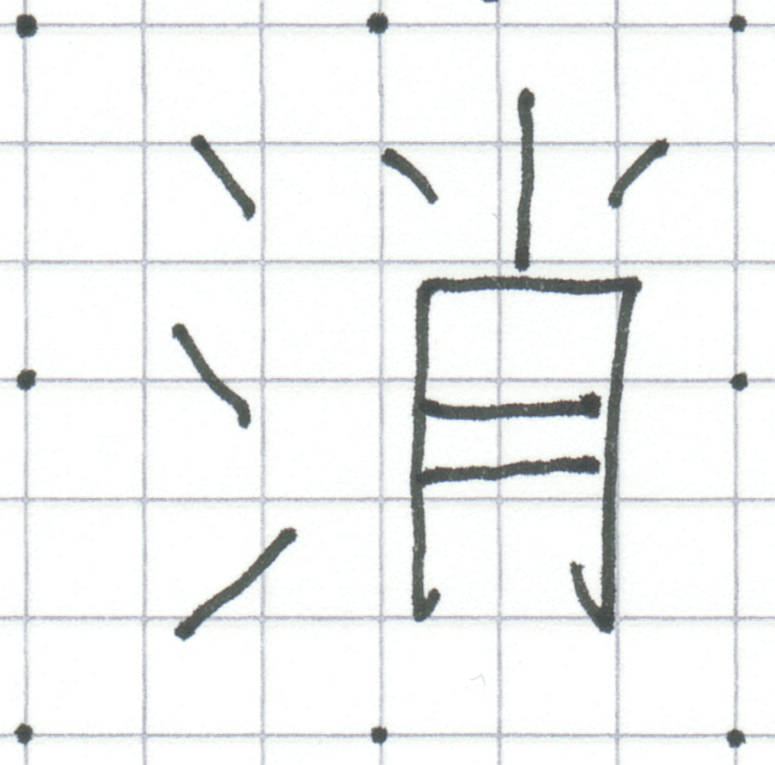
\includegraphics[scale=0.2]{images/characterMinimalBoxes1.png}
%     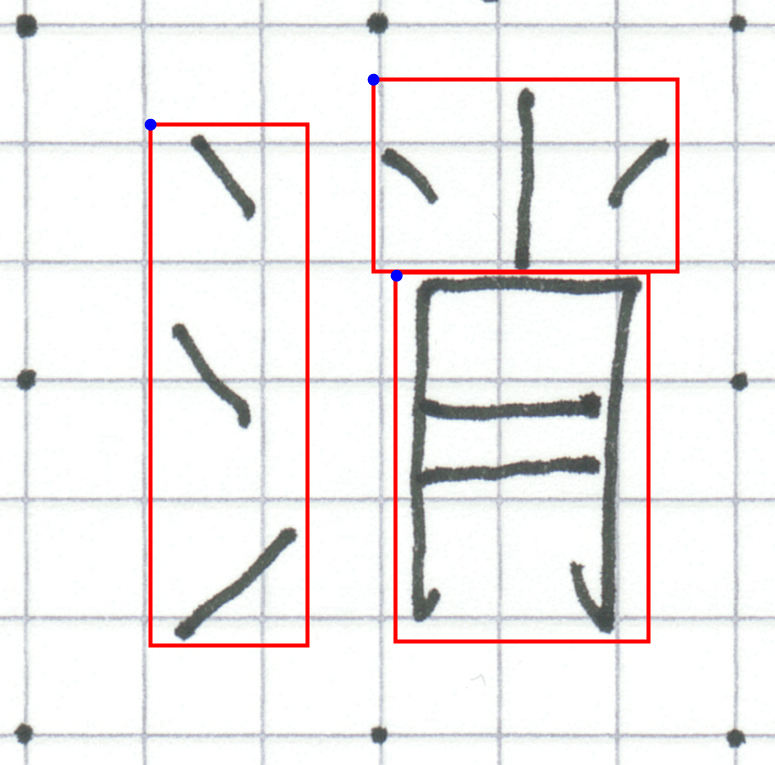
\includegraphics[scale=0.2]{images/characterMinimalBoxes2.png}
%     \caption{Minimal bounding boxes for the Radicals of the character~\cjk{消}}
%     \label{fig:boxing}
%   \end{center}
% \end{figure}

% \subsubsection{Scaling}
% \label{sec:hwre:scaling}

% The natural surrounding box of most Kanji is a square. In cases where the box
% is not a square, the space given to the Kanji by the writer in the context of
% other characters is still a square of the same size. That means, wide characters
% like \cjk{額} and narrow characters like~\cjk{月} are typically given the same 
% space by writers when they are handwriting. In typography the same is true,
% each Kanji character is given the same space, fonts that support Kanji are
% typically monospace fonts.
% In order to account for that, scaling is done with respect to the ideal of a 
% square shape of a character. That concept is used for full characters, as well
% as Radicals and strokes.
% Before scaling the size of a stroke, a square bounding box is constructed.
% The handle point of the square bounding box is used as a vanishing point for
% vectorial projection. In a stroke data structure that consists of a point
% sequence \(p_1, \ldots, p_n\)  a number of vectors 
% \(\vec{v}_1, \ldots, \vec{v}_n\) is created. Each vector is defined by the
% handle point \(H = \langle x_h, y_h \rangle \) of a square bounding box and the \(p_i\).
% \begin{quote}
% \(
%   \vec{v}_k := p_k-H = \binom{x_{p_k}-x_h}{y_{p_k}-y_h}
% \)
% \end{quote}
% In order to generate a scaled version of a sequence of points, 
% all the \(\vec{v}_k\) are multiplied with a scaling factor.
% Scaling is exemplified in figures~\ref{fig:inputandcharactermodel} 
% to~\ref{fig:inputscaledboundingbox}. 
% Figure~\ref{fig:inputandcharactermodel} shows the potential
% size difference for a character model in the database and a user input.
% Figure~\ref{fig:inputsquareboundingbox} presents the construction of a square
% bounding box from the input, via the temporary construction of a minimal 
% bounding box.
% The result of the scaling is depicted in 
% figure~\ref{fig:inputscaledboundingbox}, where the character model and the user 
% input share the same square bounding box size.
% In that state the point sequences are ready for the next step in the
% recognition process.

% \begin{figure}[htbp]
%   \begin{center}
%     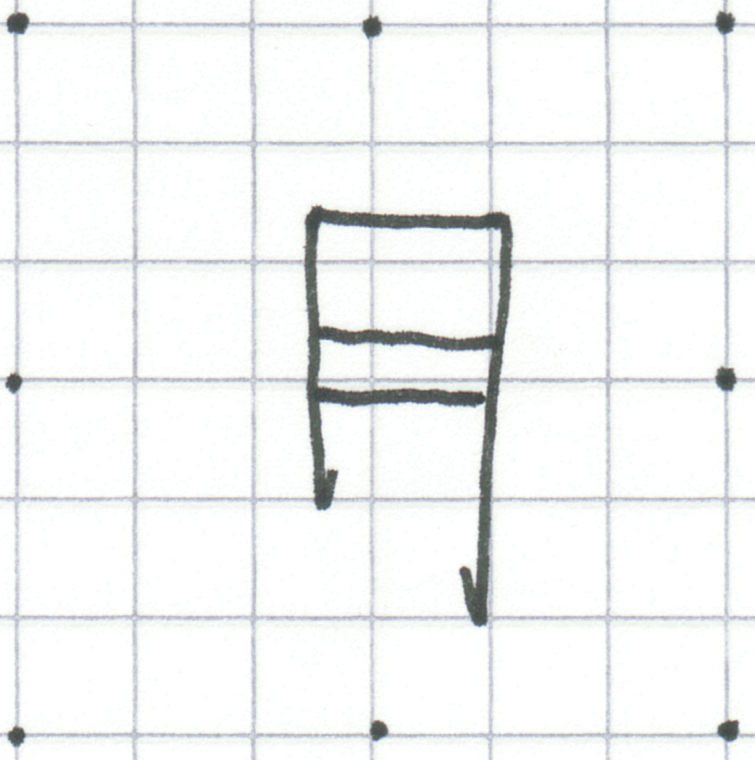
\includegraphics[scale=0.2]{images/characterModel.png}
%     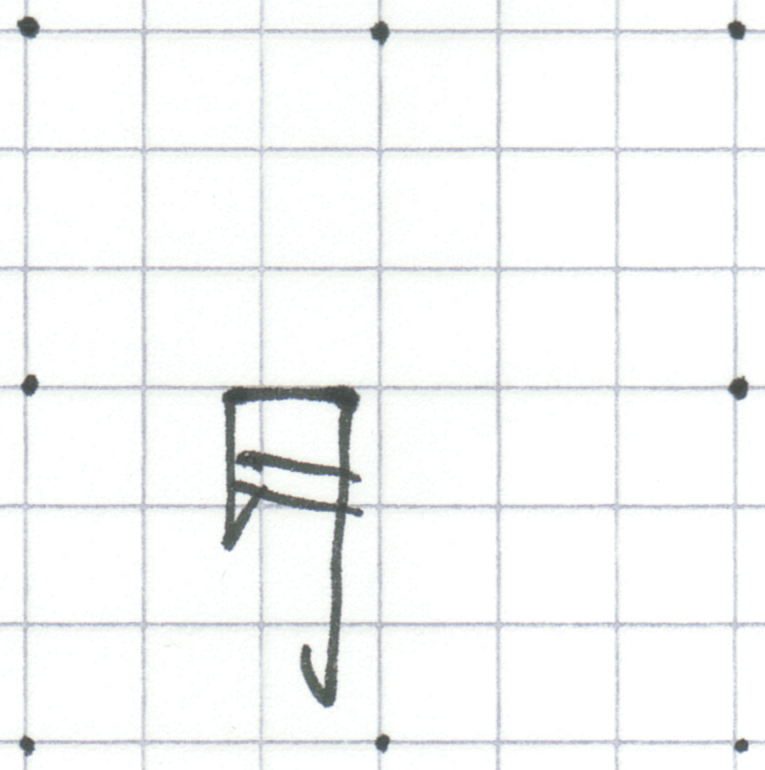
\includegraphics[scale=0.2]{images/input1.png}
%     \caption{A character model (left) and a user input (right) in their original size.}
%     \label{fig:inputandcharactermodel}
%   \end{center}
% \end{figure}
% \begin{figure}[htbp]
%   \begin{center}
%     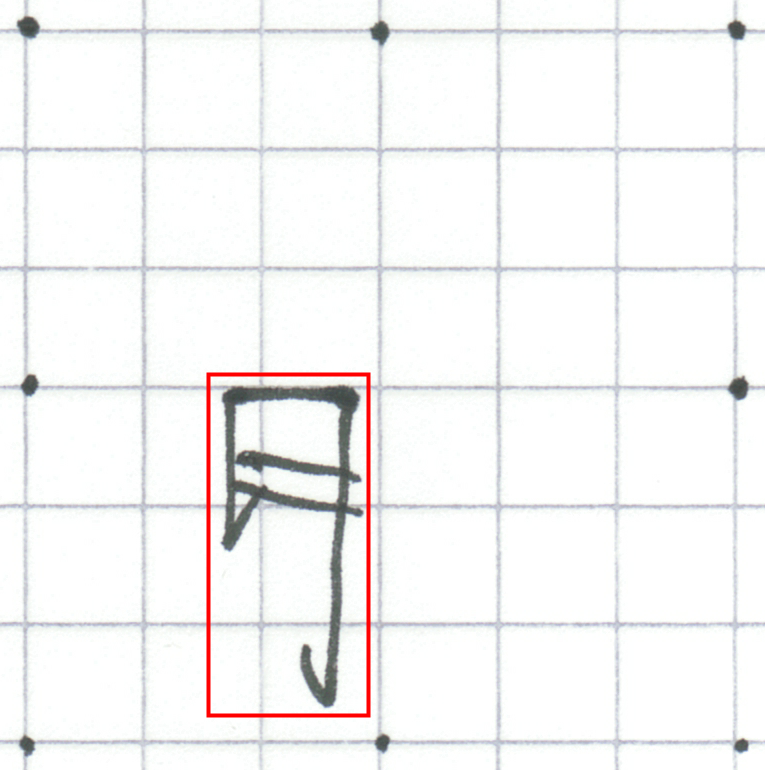
\includegraphics[scale=0.2]{images/input2WithMinimalBoundingBox.png}
%     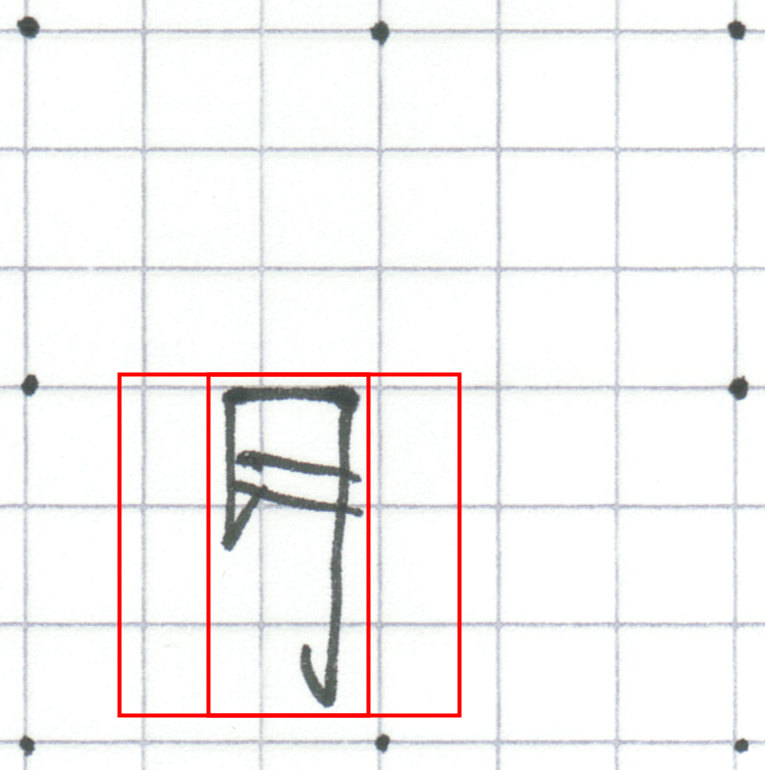
\includegraphics[scale=0.2]{images/input3WithSquareBoundingBox.png}
%     \caption{Construction of a square bounding box (right) from the minimal bounding box (left).}
%     \label{fig:inputsquareboundingbox}
%   \end{center}
% \end{figure}
% \begin{figure}[htbp]
%   \begin{center}
%     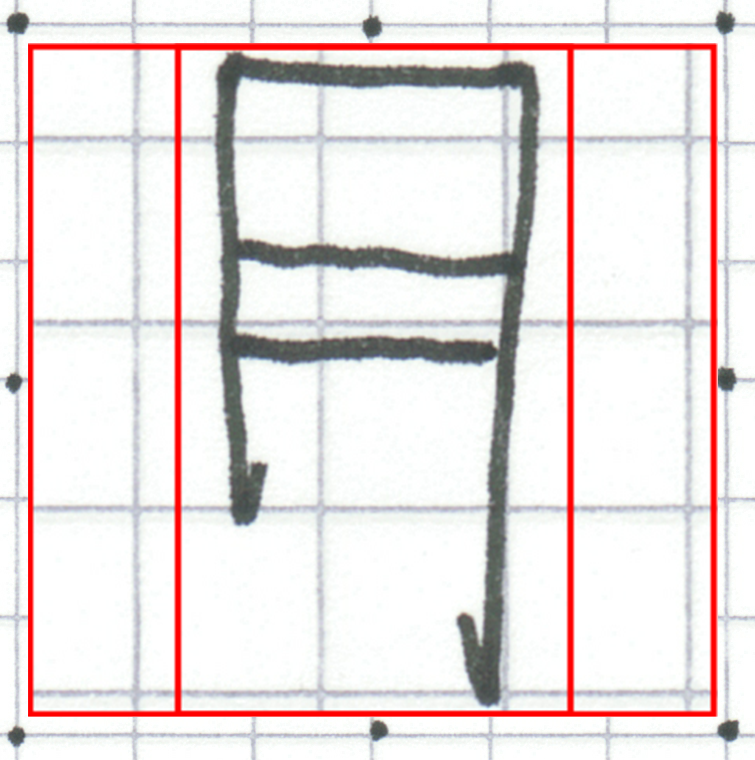
\includegraphics[scale=0.2]{images/characterModelScaled.png}
%     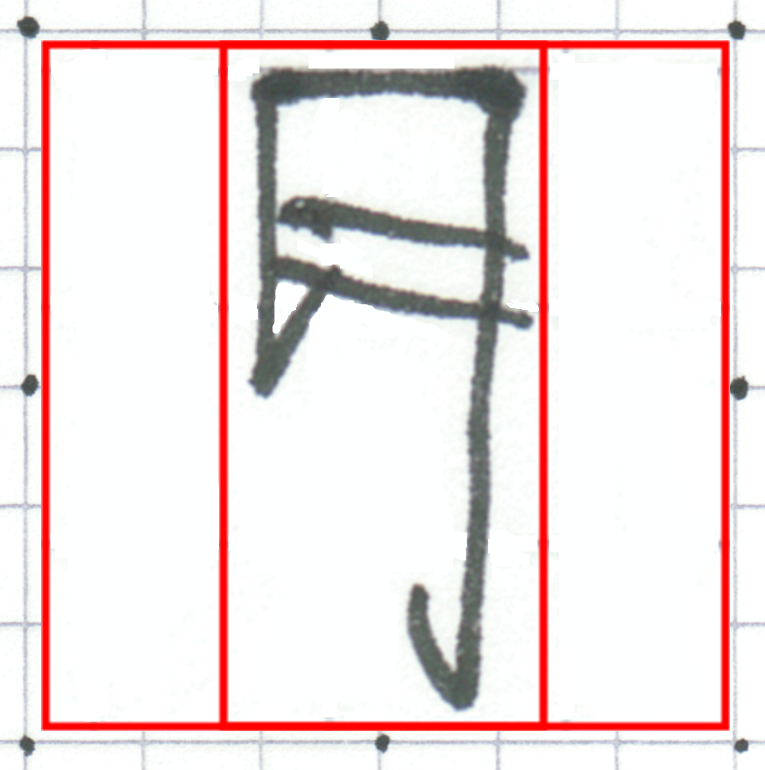
\includegraphics[scale=0.2]{images/input4WithScaledBoundingBox.png}
%     \caption{Character model (left) and user input (right) scaled to the same square bounding box size.}
%     \label{fig:inputscaledboundingbox}
%   \end{center}
% \end{figure}

% \subsection{Recognition of Straight Strokes}
% \label{sec:hwre:straightstrokes}

% \subsubsection{Identification of a Straight Stroke}
% \label{sec:hwre:identificationstraightstroke}

% The notion of \emph{stroke} essentially means \emph{point sequence} in a 
% technical sense. That is, strokes are not mathematical objects like functions.
% In order to perform stroke recognition, it is necessary to determine what shape 
% a stroke has. For the identification of a straight stroke, a linear regression 
% line is constructed from the point sequence with the Gaussian method of 
% least squares. The construction is done with the standard method for 
% calculating least squares, as described in literature. The method seeks for the 
% minimal sum of squares of residuals~\shortcite{Marquardt1963}. 
% If the sum of residual squares is below 
% a certain threshhold that has been determined empirically, 
% the system assumes that the point 
% sequence generally follows a straight line. In that case, straight stroke 
% matching will be performed. If the line appears to be curved, it will be matched
% with curve analysis methods as described in 
% section~\ref{sec:hwre:curvehandling}. 

\subsubsection{Straight Stroke Matching}
\label{sec:hwre:straightstrokematching}

For the matching of a straight stroke there are a number of features
that could be considered for a feature vector.
In order to describe a straight stroke and then match it with another one,
a feature vector is constructed that has the following features:
\begin{itemize}
  \item \textbf{Length}: The total length of the line. Sum of the distances of
        succeeding points.
  \item \textbf{Initial point}: The coordinates of the initial point
  \item \textbf{Endpoint}: The coordinates of the endpoint
  \item \textbf{Total number of measured points}: The number of sample
        points that were measured by the input device
  \item \textbf{Velocity}: The velocity with which the stroke was drawn
%  \item \textbf{Sum of residual squares}: The sum of residual squares of the 
%        points, relative to a straight line
  \item \textbf{Gradient}/\textbf{Direction}: The slope of the linear 
  regression line that can be constructed for the point sequence, or
  the general direction of the line, represented as a numerical vector.
\end{itemize}
In the following, the index \emph{db} will be used for values that are
stored in the database or have been constructed from values that are stored
in the database. Likewise, the index \emph{exp} will be used for any 
input values and values constructed from them. The variable \emph{l} 
will be used for the total lenght of a stroke, \(P_{I}\) will be the 
initial point, and \(P_{E}\) will be used for the endpoint of a stroke. 
A vector that indicates the general direction of a straight stroke will be 
called \emph{direction vector} and denoted as~\(\vec{d}\). A linear regression 
line that is constructed with the sum of residual squares method 
will be denoted as~\(f\).
In order to match two strokes by their feature vectors \(F_{db} \) 
and \(F_{exp} \), the following values are considered:
\begin{quote}
\(
    F :=
    \left( 
    \begin {array} {l c} 
%        \text{Total number points} & n_{p} \\
        \text{Length} & l \\
        \text{Initial point} & P_{I} \\
        \text{Endpoint} & P_{E} \\
        \text{Velocity} & v \\
        \text{Direction vector} & \vec{d} \\
        \text{Regression line} & f \\
    \end {array} 
    \right)
\)
\end{quote}
The features are used for matching with other straight strokes by comparison
of their values. 
The length \(l\) is calculated as the sum of the Euclidean distances \(d_i\) 
between the individual points \(P_i\) and \(P_{i+1}\) within a sequence 
of \(N\) points. Concretely, \(d_i\) equals the distance between
\(P_i\) and \(P_{i+1}\).
\begin{quote}
\(
    d_i := \sqrt{(x_{i+1}-x_{i})^2+(y_{i+1}-y_{i})^2}\\
    l := \sum\limits_{i=1}^{N-1}{d_i}
\)
\end{quote}
In the case of the initial point and endpoint comparison of the two strokes, 
the Euclidean distance between the database points \(P_{I,db}\) and \(P_{E,db}\)
and the candidate points \(P_{I,exp}\) \(P_{E,exp}\), repectively is used as a 
comparison value. 
Theoretically, this distance could also be used as the total length
of the stroke, however, since this shortest possible length value is 
already exploited in this way, the \emph{drawn length} should be exploited 
in another way. That is the main reason for defining the length the way as
the sum of the between-point distances.

The velocity \(v\) is calculated from the time 
difference \( \delta_T \) between 
\emph{sampling time of the initial point}~\(t_{p_I}\) and the 
\emph{sampling time of the endpoint} \(t_{p_E}\):
\begin{quote}
\(
    \delta_T :=
        t_{p_E} - t_{p_I}
\)
\end{quote}
\begin{quote}
\(
    v := \frac{l}{\delta_T}
\)
\end{quote}
The velocities \(v_{db}\) and \(v_{exp}\) are both real numbers and can be 
compared directly.
It is important to note that the featured direction vectors~\(\vec{d}_{db}\) 
and~\(\vec{d}_{exp}\) are the direction vectors of the regression line of the
point sequence. They are compared by the deviation of their directions.
The deviation is expressed as the angle \( \alpha \) between the 
original vector~\(\vec{d}_{db}\) and the candidate vector~\(\vec{d}_{exp}\).
\begin{quote}
\(
    \alpha := \vec{d}_{db} \quad \angle \quad \vec{d}_{exp}
\)
\end{quote}
The comparisons between the regression lines is not a direct comparison.
The computation assumes that the regression lines are identical or at least 
very similar. That may or may not be the case.
The comparison value \(s_{r}\) is calculated as a sum of residual 
squares of the candidate point sequence with respect to the regression line 
of the database point sequence.
Given the regression line \(f_{db}\), the sum of residual squares for the 
input sequence is:
\begin{quote}
\(
    s_{exp} := \sum\limits_{i=1}^{N}{(f_{db}(x_{i,exp}) - x_{i,exp})^2}
\)
\end{quote}
The smaller \(s_{exp}\) the closer the measured points to the regression line
from the database. The calculation is only done one way. The other way,
calculating \(s_{db}\) the sum of residual squares of the database point sequence
with respect to the regression line of the input point sequence \(f_{exp}\)
will not be used.
Generally, this sum is only calculated for strokes that have been found
to be straight. Any set of points can have a linear regression line, 
even curved ones. In the case of curved strokes, a linear regression line as 
it is used here does not seem to bear the potential helping identify a point 
sequence to be a certain shape.

\subsection{Curve Handling}
\label{sec:hwre:curvehandling}

\subsubsection{Detecting Curves in Strokes}
\label{sec:hwre:detectingcurvesinstrokes}

Different curve matching techniques are described in 
section~\ref{sec:curvematching}. The technique used here refers to is a 
vector-based technique, that aims at the extraction of features to describe
the curved stroke. In this prototype the direction feature plays a crucial role.
It is generally following several approaches in on-line handwriting recognition
literature. The direction feature as it is used in other applications has been
discussed in section~\ref{sec:strokedirection}). The approach for curve
recognition used here defines direction vectors.

The general concept is to define a direction vector between a point
within the point sequence and a successor point.
However, since the measured points are usually very close together, 
the direction vector is defined between a point and another point that 
is further away, defined by a dynamic threshold, considering distance,
total number of points and the total length of the stroke.
If non of these vectors deviates from the general direction of the stroke,
a dynamic threshold, considering the total stroke length,
the stroke is considered straight. Nevertheless, for matching straight strokes,
a feature vector for straight strokes is used.
If the slope of the curve changes, i.e., the direction of the vectors changes, 
a curve has been detected. 
There is a threshold \( T_{min} \) for the minimal size of a 
\emph{recognisable angle} between two vectors. Any angle smaller than that will 
be ignored completely. A second threshold \( T_{max} \) describes the minimal size
for an angle \( \gamma \)  that is taken into account.
Any angle \( \beta_{i} \) between \( T_{min} \) and \( T_{max} \) will be stored. 
When the sum of the \( \beta_{i} \) exceeds \( T_{max} \) the position will be 
treated as a curve.

\begin{quote}
\(
  \alpha < T_{min} \Rightarrow \alpha \text{ will be ignored}
\)
\end{quote}
\begin{quote}
\(
  T_{min} < \beta_{i} < T_{max} \Rightarrow \beta_{i} \text{ will be stored}
\)
\end{quote}
\begin{quote}
\(
  T_{max} < \gamma \Rightarrow 
                  \gamma \text{ will be interpreted as an angle in the stroke}
\)
\end{quote}
\begin{quote}
\(
  T_{max} < \sum\limits_{i=k}^{l} \beta_{i} \Rightarrow 
                               \sum\limits_{i=k}^{l} \beta_{i}
                               \text{ will be interpreted as an 
                               angle in the stroke}
\)
\end{quote}
A successful curve detection extracts the key feature of the curve 
description. The remaining features can be extracted or calculated,
by using the detected curves.

\subsubsection{Feature Extraction for Curved Strokes}
\label{sec:hwre:featureextractionforcurvedstrokes}
xxx die variablen einfuehren.
The feature vector for curved strokes contains the following elements:
\begin{quote}
\(
    F :=
    \left( 
    \begin {array} {l c} 
        \text{Length} & l \\
        \text{Initial point} & p_{I} \\
        \text{Endpoint} & p_{E} \\
        \text{Velocity} & v \\
        \text{Corner angles} & \gamma_{i} \quad i := 1, \ldots , n \\
        \text{Corner points} & c_{i} \quad i := 1, \ldots , n \\
        \text{Direction sequence} & \vec{d}_j \quad j := 1, \ldots , m \\
    \end {array} 
    \right)
\)
\end{quote}
The partial feature vector \( l, p_{I}, p_{E}, v\) is identical to the partial
feature vector of the straight strokes with the same elements and needs no
further description (see section~\ref{sec:hwre:straightstrokematching}).
The corner angles have been calculated. In the case of a summation
of angles the point with the greatest angle will be determined as the 
corner point. In the case of angles that have been observed directly without 
summation, the corner point is the point where the angular vectors meet.
Therefore, the number of corner points \( m \) and corner angles is identical.
The feature \emph{Corner points} is defined as the sum of Euclidean distances 
between the corner points from the stored data structure with the candidate 
data structure.
\begin{quote}
\(
%  d_i := 
  c_p := \sum\limits_{i=1}^{n} \sqrt{(x_{i,db}-x_{i,exp})^2+(y_{i,db}-y_{i,exp})^2} % d_{i} 
\)
\end{quote}
The corner angles feature is defined as the sum of the squares of the 
differences between the angles at the corner points.
\begin{quote}
\(
  c_a := \sum\limits_{i=1}^{n} (\beta_{i,db}-\beta_{i,exp})^2
\)
\end{quote}
For both \( c_a \) and \( c_p \) the smaller the value, the closer the more
similar the strokes. In fact, if \( c_a \) or \( c_p \) are equal to \(0\),
the point analysed point sequence was identical with the stored point sequence.
The \emph{direction sequence} feature takes into account all the direction 
changes, as opposed to the corner angles that use only the most significant ones.
The direction sequence feature uses the angle of each line segment regarding the 
X-axis of the coordinate system. The angles are then matched against the time
they were produced in.
%xxx how is this done exactly? what if the number of points differs?
%how is the time involved?
%S 14, 16, 17
%how is curver handling done?
%show requirements.
%what alternatives were there to consider?
%
%stroke matching with angles instead of point position.
%s. 24

\subsection{Dynamic Time Warping}
\label{sec:hwre:dynamictimewarping}

The technique of \emph{dynamic time warping} (DTW) has been used for stroke 
matching by several studies and systems (see sections~\ref{{sec:curvematching}} 
and~\ref{sec:olccr:structuralclassification}).
It is an elastic matching technique that seeks an optimal path through
a matrix of point distances. Details of the algorithm have been described
in literature.

\subsubsection{Standard DTW}
\label{sec:hwre:standarddtw}

Following~\shortciteANP{Vuori2001}~\citeyear{Vuori2001} 
and~\shortciteANP{Niels2005}~\citeyear{Niels2005}, 
the DTW technique is implemented for two pen trajectories, 
namely the trajectory stored in the database 
\(P_{db} = (p_{1,db}\ldots,p_{n,db})\) and the input trajectory generated by
the user's drawing \(P_{exp} = (q_{1,exp},\ldots,q_{m,exp})\).
Any point pair \(p_{i,db}\) and \(p_{j,exp}\) matches if one of two constraints 
is met:
\begin{enumerate}
  \item \textbf{Boundary condition}: The points \(p_{i,db}\) and \(p_{j,exp}\)  
         match, if one of the following boundary conditions is fulfilled:
        \begin{itemize}
          \item \(p_{i,db}\) equals the initial point \(p_{I,db} \) 
                and \(p_{j,exp}\) equals the initial point \(p_{I,exp}\)
                of their respective point sequences \(P_{db}\) or \(P_{exp}\)

          \item \(p_{i,db}\) equals the endpoint \(p_{E,db} \) 
                and \(p_{j,exp}\) equals the endpoint \(p_{E,exp}\)
                of their respective point sequences \(P_{db}\) or \(P_{exp}\)
        \end{itemize}

  \item \textbf{Continuity condition}: The points \(p_{i,db}\) and \(p_{j,exp}\)  
         match, if the following equation is fulfilled \\
         \begin{quote}
         \(
            \frac{M}{N}i - cM \le j \le \frac{M}{N}i + cM
         \)
         \end{quote}
         \(c\) is a constant between \(0\) and \(1\), indicating the 
         strictness of the condition.
\end{enumerate}

\subsubsection{3-Dimensional DTW}
\label{sec:hwre:3ddtw}

In addition to the standard DTW algorithm, a second DTW classifier performs 
a 3-dimensional distance calculation.
That is, a point sequence \(P = (p_{1}\ldots,p_{n})\) is considered 
3-dimensional in the way that it contains the relative time (in ms) from the
beginning of the stroke as a third dimension.
The point distance calculations are Euclidean, ignoring the fact that the
third dimension is a different type of coordinate.
\begin{quote}
\(
  d_i := \sqrt{(x_{i,db}-x_{i,exp})^2+(y_{i,db}-y_{i,exp})^2+(z_{i,db}-z_{i,exp})^2} 
\)
\end{quote}
\(\langle x_i, y_i \rangle \) are the regular 2-dimensional point coordinates, 
while the \(z_i\) are the relative times from the beginning of the stroke.
The actual DTW algorithm works exactly the same, the difference lies in 
the distance calculation.
This version of the algorithm has been conducted as an experiment. The direct
comparison with the regular DTW is reported in 
section~\ref{sec:impl:dtwvs3ddtw}.
% what's the similarity measure for
% points and strokes?
% show requirements.
% what alternatives were there to consider?

% s. 51
% how is dynamic time warping done here?
% pointer to papers or hwr - chapter, don't explain DTW here.
% show requirements
% why DTW?
% what alternatives were there to consider?
% none - it is the alternative.
% to all the other stuff I've been doing.
% however, what about 3D time warping?

\subsection{Stroke Matching Summary}
\label{sec:hwre:strokematchingsummary}

Four different classifiers have been implemented.
The straight stroke matching via regression lines,
the curve matching classifier with direction sequences and two variants
of the dynamic time warping algorithm, a regular DTW algorithm and the 
three-dimensional variant DTW.
The stroke matching occurs in NUMBER parts. 
Firstly, the straight stroke recogniser attempts to establish if a stroke 
is straight or not. Then the straight stroke matcher analyses if the input
stroke and the database stroke are equal.
Secondly, if the stroke is regarded as being curved, the curve detector 
performs a search for the significant points and angles in both sequences.
After that, the curved stroke matcher compares the features of the curved
strokes. If both recognisers fail to recognise the expected stroke, 
dynamic time warping is used as a fall-back option.

\section{Radical Recognition Process}
\label{sec:hwre:radicalrecognitionprocess}

\subsection{Radical Recognition Features}
\label{sec:hwre:radicalrecognitionfeatures}

The recognition of a Radical is a search process. The data format of Radicals is 
described in section~\ref{sec:hwre:radicaldataformat}.
Essentially, a Radical is an ordered collection of strokes.
In order to recognise a radical, the sequence of strokes from the database
is compared to an input sequence.
The measure of similarity is a feature vector that consists of the number of
strokes and the similarities between them.
Furthermore, permutations of the stroke sequence will be penalised.
In order to match two radicals by their feature vectors \(F_{db} \) 
and \(F_{exp} \), the following values are considered:
\begin{quote}
\(
    F :=
    \left( 
    \begin {array} {l c} 
        \text{Total number of strokes} & n_{s} \\
        \text{Position of bounding box} & P \\
        \text{Size of bounding box} & S \\
        \text{Stroke matching values} & m_{i,j} \\ 
        \text{Stroke sequence} & \langle s_1,\ldots,s_n \rangle  \\
    \end {array} 
    \right)
\)
\end{quote}
Some of the features need little explanation. The total number of strokes 
\( n_{s} \) is an integer. In the matching process - if the \(n_{s,db} \) and
\(n_{s,exp} \) differ, the confidence value of the radical recognition value 
will be lowered. The position of the bounding box \(P\)is determined by the 
handle point of the box. The Euclidean distance between the \(P_{db}\) and 
\(P_{exp}\) serves as a distance measure. The size of the bounding box \(S\) 
can support or refute assumptions about the general shape and size of a radical.

\subsection[Exploitation of Stroke Recognition]
{Exploitation of the Stroke Recognition Process}
\label{sec:hwre:exploitationofstrokerecogition}

Stroke matching forms the core of the Radical recognition process.
Each input stroke is matched against all the strokes of the Radical. 
A matrix of matching values will be generated by comparing each input stroke 
to each database stroke for a Radical.
The confidence values in the stroke matching matrix \(M\) are used to analyse 
if the input stroke sequence signifies the currently analysed Radical.
\begin{quote}
\(
 M_{m,n} = 
 \begin{pmatrix}
  \mu_{1,1} & \mu_{1,2} & \cdots & \mu_{1,n} \\
  \mu_{2,1} & \mu_{2,2} & \cdots & \mu_{2,n} \\
  \vdots  & \vdots  & \ddots & \vdots  \\
  \mu_{m,1} & \mu_{m,2} & \cdots & \mu_{m,n} 
 \end{pmatrix}
\)
\end{quote}
The matrix \(M\) forms the basis of the Radical recognition. The maximal 
confidence value for a Radical will be achieved if
\begin{itemize}
  \item \( m = n \) 
  \item the maximal matching value \(\mu_{i,j}\) for each stroke is above a
        threshold in order to conclude that it matched with its corresponding 
        stored stroke from the database.
  \item the maximal matching values \(\mu_{i,j}\) for all strokes form a diagonal 
        path through the matrix, with \( i = j \) for each maximal matching 
        value, starting at \(\mu_{1,1}\), ending at 
        \(\mu_{n,n}\) (and \(m=n\)).
\end{itemize}
If two identical stroke sequences are analysed, the ideal is fulfilled.
Any deviance from these constraints will be penalised and leads to a lower
confidence value for the Radical match. The matrix is the source for both 
the features of the stroke matching values \(m_{i,j}\)) and the stroke sequence
\(\langle s_1,\ldots,s_n \rangle \). A deviance from the diagonal path means deviance from the 
ideal stroke sequence.

% - Why this section? 
%   The purpose of this section is to explain the Radical recognition process in
%   detail. It is a crucial part of the structural recognition process.
%   Therefore the purpose is evident - see purpose of chapter.

%   It would be off purpose, if there'd be too much around,
%   focus on the RRP only, nothing around.

% - What goes into this section?
%   The main content of this section is the radical recognition.
%   That contains how the model is matched to the input.
%   Incrementality of recognition, using one stroke, two strokes,
%   three strokes and so on...

%   * if describing a problem: why is the problem relevant.
%     it is a part of the structural recognition process!

%   * if describing a solution to a problem: what alternatives were
%     there to solve it, why was this solution chosen? 
%     again - part of the structural recognition process that allows for
%     interaction with the user concerning error recognition

%     what made it the best choice? was it the optimal solution?
%     here, simply the lacking of alternatives. if the recognition process
%     does not distinguish between 'shapes' and 'radicals' the error
%     handling engine would not be able to inform the user.
%     (xxx: turn this one around into a positive sentence. 
%     only through distinguishing... :xxx)
    
% - How will this section be structured and organised?
%   The organisational structure of the section will be as follows:

%     1. Representation of a radical as a stroke sequence
%     2. stroke matching, reordered stroke matching in order to find 
%        alternative radicals or radical variants, depending on the 
%        number of strokes involved in the process: stroke number, stroke sequence.

% - In what style will it be written?
%   The style of writing will be formal, showing the general algorithm.

% - Next action - what to write first?
%   The next part to write is the general algorithm as pseudocode.

% what's the similarity measure for
% radicals?
% show requirements.
% what alternatives were there to consider?

% what about stroke number and stroke sequence?
% why deal with it? can be dealt with? 
% how? why this way, why not another way?
% generally, how is radical recognition done?
% show requirements.
% what alternatives were there to consider?

\section{Character Recognition Process}
\label{sec:hwre:characterrecognitionprocess}

The character recognition process relies on the Radical recognition process.
Each character is comprised of a set of Radicals the position of their 
bounding boxes.
In order to determine if a stroke sequence represents a certain character,
firstly the individual Radicals are recognised. For character matching,
the recognised Radicals are compared with the Radicals of the character.
If they match with a confidence values above the threshold and their position 
within the character is correct and the character is recognised correctly.
Generally, the confidence value of a character depends on the confidence values
of the individual radicals and the distance and position of the bounding boxes
to the database entry. A feature vector \(F \) here is defined as:
\begin{quote}
\(
    F :=
    \left( 
    \begin {array} {l c} 
        \text{Number of Radicals} & n_{r} \\
        \text{Position of Radical bounding boxes} & 
                                   P_i \quad i = 1, \ldots, n_{r} \\
%        \text{Size of Radical bounding boxes} & 
%                                   S_i \quad i = 1, \ldots, n_{r} \\
        \text{Radical confidence values} & c_{i} \quad i = 1, \ldots, n_{r} \\
    \end {array} 
    \right)
\)
\end{quote}
The \(n_{r,db} \) and \(n_{r,exp} \) are compared numerically, as they are real 
numbers. The positions of the Radical bounding boxes \(P_{i,db} \) and 
\(P_{i,exp} \) are compared by their Euclidean distance.
%The sizes of the Radical bounding boxes \(S_{i,db} \) and \(S_{i,exp} \) are 
%compared numerically. 
The Radical confidence values \(c_i\) are averaged.
The confidence value \(C\) for a character is calculated in several steps.
The confidence value \(C_n\) for the number of Radicals is computed as follows:
\begin{quote}
\(
   C_n := 
   \begin{cases}
     \frac{n_{r,db}}{n_{r,exp}} & \quad \text{if } n_{r,db} \leq n_{r,exp} \\
     \frac{n_{r,exp}}{n_{r,db}} & \quad \text{if } n_{r,db} > n_{r,exp} \\
   \end{cases}
\)
\end{quote}
The confidence value \(C_p\) for the Radical positions is extracted from a 
matrix of Euclidean distances between the Radical handles 
\(P_{i,db} = \langle x_{i,db},y_{i,db} \rangle  \) and 
\(P_{i,exp} = \langle x_{i,exp}, y_{i,exp} \rangle  \). All the distance values \( \mu_{i,j}\) are 
computed first to generate a Matrix of Radical position distances 
\( M_{m,n}\), where
\( n = n_{r,db} \) and \( m = n_{r,exp} \).
\begin{quote}
\(
   \mu_{i,j} := \sqrt{(x_{i,db}-x_{j,exp})^2 + (y_{i,db}-y_{j,exp})^2}
\)
\end{quote}
\begin{quote}
\(
  M_{m,n} = 
  \begin{pmatrix}
   \mu_{1,1} & \mu_{1,2} & \cdots & \mu_{1,n} \\
   \mu_{2,1} & \mu_{2,2} & \cdots & \mu_{2,n} \\
   \vdots  & \vdots  & \ddots & \vdots  \\
   \mu_{m,1} & \mu_{m,2} & \cdots & \mu_{m,n} 
  \end{pmatrix}
\)
\end{quote}
The minimal value \( \xi_m \) of each line or column is chosen.
\( f_p \) is a constant factor for scaling the confidence value.
\begin{quote}
\(
  C_p := 
  \begin{cases}
    f_p \cdot \sum\limits_{i=1}^{n_{r,db}} \xi_i \quad \text{if } n \geq m \\
    f_p \cdot \sum\limits_{i=1}^{n_{r,exp}} \xi_i \quad \text{if } n < m
  \end{cases}
\)
\end{quote}
%The confidence value \(C_s\) for the size of the Radical bounding boxes 
%is computed as follows:
The confidence value \( C \) is the averaged sum of the other confidence
values. The sum consists of the confidence
values for the number of characters \( C_n\),
for the position of the Radical bounding boxes \( C_p\)
and the averaged sum of the Radical confidence values.
All partial confidence values are weighted with the \(w_i\) constants.
\begin{quote}
\(
    C := \frac{1}{3}
    (w_n \cdot C_n + w_p \cdot C_p + 
     \frac{w_c}{n_{r,exp}} \sum\limits_{i=1}^{n_{r,exp}} c_{i} )
\)
\end{quote}


% - Why this section? 
%   The purpose of this section is to distinguish the radical recognition process
%   from the character recognition process.
  
%   It would be off purpose, if too much of the radical recognition process would
%   be repeaeted. 

% - What goes into this section?
%   The main content of this section is to show the actual character recognition
%   process based on the radical recognition. 
%   it should show the plan to find the appropriate characters, given a number of
%   alternative radicals.
%   s. 9/10 pixelwolke vs.\ reihenfolge

%   * if describing a problem: why is the problem relevant.
%     the problem is not just relevant it is the final problem to solve
%     before solving the main problem of HWR.
%   * if describing a solution to a problem: what alternatives were
%     there to solve it, 
%     many different alternatives - see discussion of HWR, however,
%     the approach chosen here was the structural one/
%     why was this solution chosen? 
%     because of the possibility to interact with the recognition process
%     and reading partial results.
%     what made it the best choice? was it the optimal solution?
%     the other HWR approaches do not allow for the partial structural recognition
%     with linguistic components of characters.

% - How will this section be structured and organised?
%   The organisational structure of the section will contain
%   1. description of the process from  radical list to a character.
%   2. what if there are alternative radical lists?
%   3. what would've been an alternative solution?
%      directly going from exactly one radical list to exactly one chararcter.
%      s. 9/10 pixelwolke vs.\ reihenfolge

% - In what style will it be written?
%   The style of writing will be technical

% - Next action - what to write first?
%   The next part to write is to put the subparts into proper subsections.

% what's the similarity measure for
% characters?
% show requirements.
% s. 24 pseudocode

\section{Error Handling}
\label{sec:hwre:errorhandling}

% - Why this section? 
%   The purpose of this section is to demonstrate a crucial novelty of this 
%   HWR engline, the error handling module.
  
%   It would be off purpose, if it had to explain too much of the recognition 
%   process as such - that should've been done in other sections.
  
% - What goes into this section?
%   The main content of this section is the 'way of an error'.
%   what happens if the character that is bound to be recognised just 
%   doesn't fit?
%   so there's a stroke that's not long enough and it's position is not
%   high enough within the character.

%   * if describing a problem: why is the problem relevant.
%     the problem is relevant for a learning application.
%     the purpose of the application is to teach the characters with an automated
%     recognition engine - one the central ''A.I.'' of this application
%     is the automated error recognition.

%   * if describing a solution to a problem: 
%     what alternatives were there to solve it, 
    
%     the alternative to the chosen process was a less flexible approach.
%     just measuring the absolute match - in size, shape pixel by pixel
%     (again pixelwolke) would've been of a lower quality.
%     compare skritter - it does not provide the high quality feedback.

%     why was this solution chosen? 
%     because the design of the application required high-quality feedback,
%     on a linguistic level.
    
%     what made it the best choice? 
%     because it was the only one that met the requirement of providing 
%     high-qualitiy feed-back.
    
%     was it the optimal solution?
%     who knows? - looks like it now, but evaluation will show.
%     depends on user experience. 

% - How will this section be structured and organised?
%   The organisational structure of the section 
%    
%    1. error recognition
%    2. The Way of an error after recognition (error processing)
%    
% - In what style will it be written?
%   The style of writing will be a technical description - probably no algorithms

% - Next action - what to write first?
%   The next part to write is to describe the error recognition.

Error handling is a crucial part of the handwriting recognition engine.
It provides the information needed in order to give informed feedback to 
the user, when he has drawn a character. The general motivation for error 
handling has been discussed in 
section~\ref{sec:concept:motivationforerrorrecognition}
typical sources of error have been described in 
section \ref{sec:concept:sourcesoferror}. 
The focus in this section lies on the technical aspects of error handling.

\subsection{Error Detection}
\label{sec:hwre:errordetection}

% what?
% how?
% when?
% where?

% why this section? to demonstrate own achievements of error recognition.
% the reader should know how it is done technically.

% what goes into this section? the aspects of finding errors. finding errors
% is not a straightforward trivial task - whenever something does not match
% it is an error - doesn't work like that. instead, 
% firstly, it needs to be made sure that it actually is an error.
% meaning - not a recognition error, but a user error.
% secondly, the type of error needs be identified.
% see section \ref{sec:concept:sourcesoferror} (or handwritten page 58)
% for sources of error.

% how will this section be written?
% technical - first describe how the error recognition integrates into the
% recognition process, then how errors are identified.

Error detection is fully integrated into the character recognition process.
Concerning abstract module structure it is not an individual model, but rather
an integral part of the recognition module.
There is a logical explanation for that matter. The error detection in this 
prototype is a structural error analysis. The achievement of a structural error 
analysis the main cause for the character recognition process to be structural.
The task of error detection is not trivial, since there can be recognition errors
as well. However, in the case presented here, the error detection uses the
confidence value calculations for strokes, radicals and characters in order
to find out if there were errors. Additionally, the confidence values
for the structural elements define what type of error has been detected.

\subsubsection{Direction of Error Detection}
\label{sec:hwre:directionoferrordetection}

Error detection is performed when the learning system asks the user to enter a
certain character. Depending on the confidence value for the recognition of 
character substructures, error detection determines why and where the 
recognition failed. Error detection works in two directions:
From \emph{inside out} and from \emph{outside in}. 
The direction of error detection refers to the hierarchical nature of the 
character structure as well as the character recognition process.

\paragraph{Inside out} error detection occurs if the confidence value of a 
terminal element in the hierarchy was low during its recognition. 
If a stroke has been recognised as the correct stroke, but has a significant 
deviation from the corresponding stroke in the database, the deviation and 
certain information connected to it is stored as a minor error.
For example, if a straight stroke has been detected with the correct position
and the correct direction, but incorrect length, the fact that the stroke
did not have the correct length will be stored. Inside out error detection
is performed during the recognition process focuses on detecting minor errors.

\paragraph{Outside in} error detection occurs if the confidence value of a 
character was below the threshold. The cause of the low confidence value will be 
ascertained top down, checking the confidence values of the substructures.
If a character recognition failed because of a low confidence value of
a specific Radical, that Radical will be examined further.
Outside in error detection is performed after the recognition process is 
completed and focuses on detecting the major errors.

\subsection{Error Processing}
\label{sec:hwre:errorprocessing}

%focus on technical aspects
After the error detection and localisation, a feedback is generated 
depending on the primary source of the errors. Major errors contain incorrect 
characters and incorrect Radicals within characters.
Missing or additional strokes within Radicals are regarded es intermediate
errors. Minor errors are strokes that are recognisable but vary in shape from 
the database standard. The error location and type are returned together with 
the recognition result. In case a character incorrect and no error could be 
recognised, a standard character recognition process is performed.
In analogy to that, if a Radical within a character was deemed incorrect by
the system, the substructure undergoes a new recognition process.
In case of incorrect strokes the system generates an error description based
on the shape of the stroke.

% why this section? 
% actually the 'handling' or 'processing' aspect could be 
% described in the recognition section \ref{sec:hwre:errordetection} as well.
% so this section is only for a better overview, for document structure, 
% thematically they are the same section. thus they are put together under
% Error Handling \ref{sec:hwre:errorhandling}.

% what goes into this section?

